%%
%% Copyright 2007-2024 Elsevier Ltd
%%
%% This file is part of the 'Elsarticle Bundle'.
%% ---------------------------------------------
%%
%% It may be distributed under the conditions of the LaTeX Project Public
%% License, either version 1.3 of this license or (at your option) any
%% later version. The latest version of this license is in
%% http://www.latex-project.org/lppl.txt
%% and version 1.3 or later is part of all distributions of LaTeX
%% version 1999/12/01 or later.
%%
%% The list of all files belonging to the 'Elsarticle Bundle' is
%% given in the file `manifest.txt'.
%%
%% Template article for Elsevier's document class `elsarticle'
%% with numbered style bibliographic references

\documentclass[preprint,12pt]{elsarticle}

%% Use the option review to obtain double line spacing
\usepackage{markup}

%% Use the options 1p,twocolumn; 3p; 3p,twocolumn; 5p; or 5p,twocolumn
%% for a journal layout:
%% \documentclass[final,1p,times]{elsarticle}
%% \documentclass[final,1p,times,twocolumn]{elsarticle}
%% \documentclass[final,3p,times]{elsarticle}
%% \documentclass[final,3p,times,twocolumn]{elsarticle}
%% \documentclass[final,5p,times]{elsarticle}
%% \documentclass[final,5p,times,twocolumn]{elsarticle}

%% For including figures, graphicx.sty has been loaded in
%% elsarticle.cls. If you prefer to use the old commands
%% please give \usepackage{epsfig}

%% The amssymb package provides various useful mathematical symbols
\usepackage{amssymb}
%% The amsmath package provides various useful equation environments.
\usepackage{amsmath}
\usepackage{enumitem}
%% The amsthm package provides extended theorem environments
%% \usepackage{amsthm}

%% The lineno packages adds line numbers. Start line numbering with
%% \begin{linenumbers}, end it with \end{linenumbers}. Or switch it on
%% for the whole article with \linenumbers.
%% \usepackage{lineno}
\usepackage{lineno}
\usepackage{xcolor}
\usepackage{mdframed}
\usepackage{listings}
\usepackage[most]{tcolorbox}
\usepackage{hyperref}
\usepackage{rotating}
\usepackage{geometry}
\usepackage{array}
\usepackage{booktabs}
\usepackage{colortbl}
\usepackage{subcaption}
\usepackage{siunitx}
\usepackage{threeparttable}
\usepackage{tabularx}
\usepackage{caption}
\sisetup{
 group-separator = {,},
 group-minimum-digits = 4
}
\newcolumntype{C}{>{\centering\arraybackslash}p{1.8cm}}
\definecolor{panelgray}{HTML}{E6E6E6}
\definecolor{scenarioonehead}{HTML}{D7E8FA}
\definecolor{scenarioonebg}{HTML}{F3F8FE}
\definecolor{scenariotwohead}{HTML}{DDF1E2}
\definecolor{scenariotwobg}{HTML}{F4FBF5}
\definecolor{changehead}{HTML}{FBE4D5}
\definecolor{changebg}{HTML}{FDF5EF}
\definecolor{groupbg}{HTML}{F4F4F4}
\definecolor{totalbg}{HTML}{E3E3E3}
\definecolor{costinc}{HTML}{B00020}
\definecolor{costdec}{HTML}{1C6B2A}
\newcommand{\costincrease}[1]{\textcolor{costinc}{\textbf{#1}}}
\newcommand{\costdecrease}[1]{\textcolor{costdec}{\textbf{#1}}}
\lstset{
 basicstyle=\scriptsize\ttfamily,
 breaklines=true,
 breakatwhitespace=true,
 columns=flexible,
 keepspaces=true
}
\lstdefinestyle{prompttemplate}{
 backgroundcolor=\color{gray!6},
 frame=none,
 basicstyle=\scriptsize\ttfamily,
 numbers=none,
 breaklines=true,
 breakatwhitespace=true,
 columns=flexible,
 keepspaces=true,
 showstringspaces=false,
 captionpos=b
}
\newtcolorbox{promptbox}{%
 enhanced,
 breakable,
 colback=gray!6,
 colframe=black!35,
 boxrule=0.35pt,
 arc=6pt,
 left=6pt, right=6pt,
 top=4pt, bottom=4pt,
}
\journal{Applied Soft Computing Journal}
\emergencystretch=2em

\begin{document}

\begin{frontmatter}

%% Title, authors and addresses

%% use the tnoteref command within \title for footnotes;
%% use the tnotetext command for the associated footnote;
%% use the fnref command within \author or \affiliation for footnotes;
%% use the fntext command for the associated footnote;
%% use the corref command within \author for corresponding author footnotes;
%% use the cortext command for the associated footnote;
%% use the ead command for the email address,
%% and the form \ead[url] for the home page:
%% \title{Title\tnoteref{label1}}
%% \tnotetext[label1]{}
%% \author{Name\corref{cor1}\fnref{label2}}
%% \ead{email address}
%% \ead[url]{home page}
%% \fntext[label2]{}
%% \cortext[cor1]{}
%% \affiliation{organization={},
%% addressline={},
%% city={},
%% postcode={},
%% state={},
%% country={}}
%% \fntext[label3]{}

\title{Optimization of Empty Container Repositioning by Integrating Large Language Models and Multi-Agent Systems} %% Article title

%% use optional labels to link authors explicitly to addresses:
%% \author[label1,label2]{}
%% \affiliation[label1]{organization={},
%% addressline={},
%% city={},
%% postcode={},
%% state={},
%% country={}}
%%
%% \affiliation[label2]{organization={},
%% addressline={},
%% city={},
%% postcode={},
%% state={},
%% country={}}

\author[dlmu]{Kangzhen Peng}
\ead{pengkangzhen@dlmu.edu.cn}

\author[djtu]{Shida Xu}
\ead{xushida@djtu.edu.cn}

\author[nbu]{Yuhong Wang}
\ead{wangyuhong@nbu.edu.cn}

\author[sinotrans]{Mengying Hua}
\ead{huamengying@sinotrans.com}

\author[dlmu]{Zhihong Jin\corref{cor1}}
\ead{jinzhihong@dlmu.edu.cn}
\ead[url]{https://orcid.org/0000-0003-4342-1561}

\cortext[cor1]{Corresponding author. Tel.: +86; fax: +86.}

%% Author affiliation
\affiliation[dlmu]{organization={College of Transportation Engineering, Dalian Maritime University},
 addressline={No. 1 Linghai Road},
 city={Dalian},
 postcode={116026},
 state={Liaoning},
 country={China}}

\affiliation[djtu]{organization={College of Economics and Management, Dalian Jiaotong University},
 addressline={},
 city={Dalian},
 postcode={116028},
 state={Liaoning},
 country={China}}

\affiliation[nbu]{organization={Faculty of Maritime and Transportation, Ningbo University},
 addressline={No. 169, Qixing South Road},
 city={Ningbo},
 postcode={315211},
 state={Ningbo},
 country={China}}

\affiliation[sinotrans]{organization={Sinotrans Limited},
 addressline={No. 85 Renmin Road},
 city={Dalian},
 postcode={116001},
 state={Liaoning},
 country={China}}

%% Abstract
\begin{abstract}
%% Text of abstract
The problem of empty container repositioning is a core challenge within the container supply chain domain. This study addresses the limitations of existing solvers that depend on manual modeling and problem-specific customization by designing SOP-MAS (Standard Operating Procedure–Multi-Agent System), a multi-agent collaborative framework grounded in artificial intelligence large language models. This framework interprets the intricate business scenarios associated with the empty container repositioning problem through natural language instructions and employs the Gurobi solver to achieve end-to-end optimization. To validate the efficacy of the proposed method, benchmark tests were conducted utilizing the ComplexOR and NLP4LP datasets. The findings exhibit that our approach enhances the accuracy rate to 86.59\% in comparison to traditional baseline methods. Implementing this method for an empirical analysis within the Liaoning coastal port cluster-Northeast hinterland, the system optimized repositioning routes and decreased total costs by 12.18\%. This verifies its practical applicability in facilitating intelligent decision-making for the shipping industry. The research outcomes have the potential to offer shipping companies scalable intelligent decision support.
\end{abstract}

%%Graphical abstract
% \begin{graphicalabstract}
% %\includegraphics{grabs}
% \end{graphicalabstract}

%%Research highlights
% \begin{highlights}
% \item SOP-MAS: LLM-driven multi-agent dynamic orchestration enabling end-to-end automation from natural language to MIP modeling and solving; introduces dual-layer Verification \& Validation and exception backtracking, markedly enhancing reliability and controllability.
% \item Achieves 86.59\% accuracy on ComplexOR/NLP4LP with error rates of 1.39\%/2.91\%, substantially surpassing SPM, CoT, CoE, and OptiMUS through systematic workflow orchestration.
% \item In a real ECR case for the Liaoning coastal port cluster–Northeastern hinterland of China, total cost reduced by 12.18\%; results are interpretable and processes auditable, demonstrating industrial usability and reproducibility.

% \end{highlights}

%% Keywords
\begin{keyword}
%% keywords here, in the form: keyword \sep keyword

%% PACS codes here, in the form: \PACS code \sep code

%% MSC codes here, in the form: \MSC code \sep code
%% or \MSC[2008] code \sep code (2000 is the default)

large language model \sep multi-agent system \sep end-to-end optimization \sep mixed-integer programming \sep container supply chain \sep empty container repositioning
\end{keyword}

\end{frontmatter}

%% Add \usepackage{lineno} before \begin{document} and uncomment
%% following line to enable line numbers
\linenumbers

%% main text
%%

%% Use \section commands to start a section
\section{Introduction}
\changed{Empty Container Repositioning (ECR), the logistical challenge of repositioning surplus empty containers from locations with excess supply to locations with unmet demand, is a central problem in container supply chain management. Optimizing ECR requires multi-period, multi-node, and multi-modal transportation decisions under dynamic supply--demand imbalances, a task commonly formulated as a Mixed-Integer Program (MIP). In practice, however, translating such complex business scenarios into a correct MIP formulation is heavily dependent on domain experts, a procedure that is not only arduous and time-consuming but also results in inflexible models that inadequately respond to dynamically evolving business requirements. Despite the fact that algebraic modeling languages (e.g., AMPL, GAMS) have marginally enhanced modeling efficiency, their reliance on expert-authored algebraic expressions means they cannot bridge the gap between unstructured business descriptions and MIP formulation without human intervention.}

Recent advancements in Large Language Models (LLMs), particularly in the realms of natural language understanding and code generation, present transformative potential for the automation of the modeling process. These models' substantial in-context learning and natural language comprehension capabilities allow them to discern business intents, such as "minimize total cost" and initially generate corresponding mathematical formulations or solution code, thereby substantially reducing the complexity associated with modeling. Nevertheless, the inherent "hallucination" issue of LLMs and their lack of reliability in executing complex multi-step logical reasoning render them challenging to trust directly in operations research (OR) tasks that demand mathematical precision. As probabilistic generative models, LLMs might produce output that appear plausible but are mathematically unsound, which considerably restricts their practical application in critical decision-making systems. \changed{Empirical studies have documented characteristic failure modes of single-agent LLMs in optimization tasks: omitting decision variables or constraints that are implicit in the problem description, generating syntactically valid but logically incorrect mathematical formulations, and producing solver code that compiles yet yields infeasible or suboptimal solutions. These errors are particularly difficult to detect in the absence of an independent verification mechanism, as the same agent that generates the model is also responsible for validating it.}

To address these challenges, combining the reasoning capabilities of LLMs with the collaborative strengths of Multi-Agent Systems (MAS) offers a promising approach. MAS handle complexity through task decomposition and distributed collaboration. Against this background, this paper asks the following central question: How can an LLM-driven multi-agent framework be designed to understand practical business intents while ensuring reliability, controllability, and interpretability through workflow orchestration and internal verification across the full transition from natural language to final solutions? Addressing this question can help establish a general framework for automated and adaptive large-scale optimization. \changed{We employ the ECR problem introduced above as an empirical testbed, as its multi-stakeholder, multi-modal complexity and the dual demand for mathematical rigor and business interpretability make it a compelling representative of the class of problems that the proposed framework is designed to address.}

The contributions of this paper are threefold: 1) The introduction of workflow orchestration within LLM-driven multi-agent collaboration, shifting from static code generation to dynamic, adaptive task planning, thereby overcoming the rigid collaboration rules characteristic of traditional MAS; 2) The design of a systematic set of constraints and verification mechanisms to mitigate LLM hallucinations, thereby providing a novel technical path for the reliable application of LLMs in precision-critical computing domains through the integration of "multi-agent division of labor, standardized operating procedures, and exception backtracking mechanisms"; 3) \changed{The implementation and empirical validation of an end-to-end framework that translates natural language business descriptions into optimized solutions, demonstrated through the sea-land coordinated ECR problem faced by shipping companies in the Liaoning coastal port cluster, which achieved a 12.18\% reduction in total operational costs and thereby verifies both the method's effectiveness and its potential for the digital and intelligent transformation of the port and shipping industry.}


\section{Literature Review}
This research focuses on a category of problems that are essential and extensively applied within the field of OR: the automated modeling and resolution of MIP problems. This section provides a review of pertinent advancements that are central to this core theme, establishing the foundation for the subsequently proposed paradigm, which employs container SCM as a representative application scenario.

\subsection{Traditional MIP Solution}
The resolution of MIP problems generally adheres to a systematic OR framework that encompasses five stages. Initially, a mathematical model is constructed to abstract the real-world issue. Subsequently, an analysis of the problem's properties is undertaken to identify an appropriate solution strategy. The third stage involves the design and evaluation of algorithm performance. The fourth phase encompasses programming tasks to invoke optimization solvers and the execution of numerical simulations. Finally, the effectiveness of the solution is assessed, followed by its implementation. A core bottleneck within this framework lies in the significant dependence on experts for the laborious and time-intensive responsibilities of model development and parameter tuning.

While MIP is theoretically and algorithmically mature, its practical application encounters fundamental challenges. The modeling phase, serving as the cornerstone of the entire process, continues to present considerable difficulties. This phase necessitates experts to convert complex real-world scenarios into mathematical variables, objective functions, and constraints, which is not only resource-intensive and protracted but also significantly reliant on expert experience \citep{liLargeLanguageModels2023}. This dependency constitutes the fundamental impediment to its extensive and rapid adaptation to novel scenarios. Models developed for specific context often require expert re-evaluation and modification when business conditions alter (e.g., incorporating new warehouse capacity constraints), which suggests a limited capacity for generalization. As real-world issues increase exponentially in scale and complexity, the traditional method reliant on individual experts for modeling proves inadequate to satisfy these demands.

In response to the challenging nature of employing general-purpose programming languages for complex MIP models, Algebraic Modeling Languages (AMLs) have emerged. Prominent examples, such as AMPL and GAMS, aim to elevate the level of abstraction from procedural code to algebraic expressions, thereby decoupling models from data and enhancing modeling efficiency. \changed{These languages serve as structured intermediate representations that formalize optimization models in a solver-agnostic manner, and modern systems such as SOP-MAS can leverage them as compilation targets for automatically generated code.} In recent developments, optimization libraries grounded in general-purpose programming languages (e.g., Pyomo, PuLP) are embedded as libraries within modern high-level languages, facilitating the use of robust data science ecosystems and toolchains for the seamless integration of optimization models and solvers. \changed{More recently, knowledge- and data-driven hybrid methods have begun to automate scheduling and optimization beyond purely expert-built models \citep{zhangKnowledgeDataDriven2025}.}

Nonetheless, AMLs remain unable to automatically transform unstructured business descriptions into MIP formulations. For instance, within the context of container supply chain optimization, changes in the business environment necessitate experts to manually reinterpret new requirements, such as converting the need to "avoid empty container accumulation at ports" into balance constraints involving inventory variables. This demonstrates the significant reliance of AMLs on expert modeling. Additionally, the specific syntax of AMLs acts as an impediment for domain experts without technical backgrounds (e.g., shipping company schedulers), thus restricting the broad adoption of optimization technologies.

\subsection{Emerging Paradigms from LLMs in Scientific Computing and OR}

The emergence of LLMs in recent years brings revolutionary opportunities to the domains of scientific computing and OR. These models, trained on extensive corpora, demonstrate powerful capabilities in natural language understanding, code generation, and mathematical reasoning. LLMs offer an innovative approach to address the previously mentioned challenges. Their exceptional performance in open-domain natural language understanding significantly enhances efficacy in tasks involving arithmetic, commonsense, and symbolic reasoning. Chain-of-Thought (CoT) prompting, initially proposed by \citet{weiChainofthoughtPromptingElicits2022a}, enables models to deconstruct complex problems into multiple steps, substantially improving LLMs' reasoning ability without the need for fine-tuning, thus allowing them to tackle mathematical word problems and commonsense reasoning effectively. The introduction of CoT suggests that LLMs are also capable of resolving complex mathematical problems requiring precise, step-by-step calculation. Moreover, CoT contributes to the interpretability and reliability of LLMs. Traditionally, large-scale unsupervised deep learning models have been perceived as opaque entities with enigmatic decision-making processes, which raises concerns about the credibility of their results. By decomposing logical reasoning problems into sequentially solvable steps, CoT provides a transparent logical framework for the results generated, thus offering a level of explicability. Research based on CoT has expanded considerably. The conceptualizations of Tree of Thoughts \citet{yaoTreeThoughtsDeliberate2023a} and Graph of Thoughts \citet{bestaGraphThoughtsSolving2024a} have further enhanced reasoning capability by allowing LLMs to explore and integrate thoughts in a structured manner. These studies demonstrate the potential of LLMs in resolving complex problems, especially those involving reasoning and mathematics.

Concurrently, the utilization of LLMs in scientific computing is transitioning from proof-of-concept to practical application, showing growing potential in disciplines such as computer science, transportation, logistics, and SCM. For example, in the domain of complex system simulation, \citet{liAdaptiveTODLLMdrivenAdaptive2025a} developed a natural language interface employing adaptive dialog agents that comprehend user intent and dynamically generate task flows, thereby demonstrating the capacity of LLMs to simplify the complexity associated with simulation modeling. In the specific context of OR, the natural language processing capability of LLMs offers a novel avenue to overcome the modeling bottleneck associated with MIP. Taking the representative MIP problem of vehicle routing as an example, \citet{jiangDROCELEVATINGLARGE2025a} noted that LLMs are capable of precisely translating business descriptions such as "minimize total transportation cost," "ensure inventory balance across warehouses," or "meet customer time window constraints" into structured decision variables, objective functions, and constraints. This capacity provides strong support for rapid prototyping and model iteration, thereby significantly enhancing modeling efficiency. \citet{liuSTLLMGraphEnhanced2025} employed LLMs for traffic flow prediction, while \citet{ishibashiSelfOrganizedAgentsLLM2024} concentrated on code generation. For modeling new scenarios, LLMs have the capability to automatically generate complete optimization models and solving code on the basis of scenario descriptions provided by algorithm engineers, in consequence significantly reducing development timelines. \changed{Parallel efforts explore the integration of Transformer architectures with reinforcement learning for general decision-making \citep{yuanTransformerReinforcementLearning2024} and the fine-tuning of LLMs for combinatorial optimization \citep{liMultitypeGameOptimisation2026}, further expanding the application frontier of LLM-driven optimization.}

In spite of their considerable potential, LLMs operating as solitary agents encounter the following challenges when handling complex optimization tasks:
1) Hallucination and Uncontrollability: LLMs are inherently probabilistic generative models, and as such, they may produce code that appears plausible but is mathematically invalid, leading to challenges in ensuring the accuracy and controllability of results \citep{huangSurveyHallucinationLarge2025}.
2) Deficiency in Transparency and Interpretability: Numerous LLMs function as "black box" models, rendering it challenging to understand their decision-making processes and to verify results in critical decision-making scenarios.
3) Constraints in Multi-step Task Handling: The computational and decision-making demands placed on an individual LLM can increase dramatically when engaging with MIP tasks that necessitate complex, multi-step reasoning and planning \citep{labanLLMsGetLost2025a}.


\subsection{Distributed Collaboration and Optimization in MAS}

In response to the constraints associated with LLMs, researchers have commenced investigations into technical pathways that integrate LLMs with MAS. The latter can effectively handle complex problems by leveraging multiple autonomous, interacting agents working collaboratively. Research focusing on LLM-based multi-agent collaboration has revealed that dynamic interaction, characterized by both cooperation and competition, frequently leads to unanticipated efficacy. \citet{wuAutoGenEnablingNextGen2024} proposed the AutoGen framework to facilitate the implementation of LLM applications through the configuration of multiple agents. Empirical studies have demonstrated the framework's effectiveness across diverse applications, such as mathematical problem-solving and coding, conversational question answering, operational optimization, and online decision-making. \citet{hongMetaGPTMetaProgramming2023a} introduced Standard Operating Procedures (SOP) into MAS to facilitate software development. Within the domain of operations optimization, existing studies have engaged LLMs in addressing problems such as linear programming and MIP. For example, \citet{zhangNeuralTSPSolver2023} attempted to resolve the Traveling Salesperson Problem utilizing LLM based reasoning, demonstrating commendable performance on small-scale instances. \citet{ramamonjisonNL4OptCompetitionFormulating2023} introduced the NL4Opt competition, which aimed at the extraction of meaning and formulation of optimization problems derived from natural language, involving sub-tasks of identifying semantic labeling and generating logical representations. The competition has the potential to enhance the interactive capability between non-expert users and optimization solvers. \citet{ahmaditeshniziOptiMUSScalableOptimization2024b} designed a system intended for formulating and resolving (Mixed Integer) Linear Programming problems based on natural language descriptions. This system is proficient in developing mathematical models and writing debugging solver code. \citet{xiaoChainofExpertsWhenLLMs2023} devised a multi-expert collaboration framework, known as Chain-of-Experts (CoE), aimed at automating the modeling and programming process for complex OR problems, ultimately diminishing dependency on domain-specific experts. Experimental results showed that CoE significantly outperformed state-of-the-art LLM methods in terms of performance on both LPWP and ComplexOR benchmarks.


\subsection{Overview of Empty Container Repositioning Challenges}

The issue of ECR presents a significant challenge within the domain of the container supply chain, and has long been an important research topic in academia. \changed{The broader trend of supply chain digitalization \citep{huImpactSupplyChain2026} further accentuates the need for agile, data-driven repositioning decisions.} Traditionally, ECR research has concentrated on a single mode of repositioning between seaports via maritime routes, emphasizing the optimization of components such as ship routing \citep{xiangLinerFleetDeployment2024,xiangTacticalVesselDeployment2024,xuEmptyContainerRepositioning2024}, shipping network design \citep{kuzmiczContainerDepotLocation2020, shanExactAlgorithmInland2020, zhangTacticalOperationalCooperative2019}, and slot allocation \citep{liangDynamicContainerSlot2024} through MIP. \citet{yuPricingCompetitionMaritime2024} explored the dynamics of pricing competition in maritime transport under blockchain technology and ECR, determining perceived container leasing prices through inverse optimization methodologies. These investigations tend to disregard the particularities associated with land transport – specifically, when shipping companies utilize their own fleets, the marginal cost of sea repositioning approaches zero, starkly contrasting with the costly nature of land transport. Inland container transportation, which encompasses the terrestrial component of the transport chain, significantly drives costs in container shipping, accounting for 50\%-70\% of total container transport volume and potentially up to 40\% of total transport costs, thus constituting a critical bottleneck in the pursuit of operational optimization within the shipping sector. Research on inland ECR has gradually increased in recent years. \citet{faziMultitripContainerDrayage2023} studied a hinterland transport network consisting of a seaport and a dry port, devising an ECR model that accounts for both laden and empty container transport to minimize costs, showing that the utilization of dry ports can reduce laden container transport costs. \citet{caiJointOptimizationEmpty2024} investigated ECR patterns between port nodes and inland depot nodes within their respective zones, providing insights applicable to practical ECR challenges. As inland dry ports evolve, they, alongside seaports, form intermodal systems facilitated by railway collaboration; however, these entities frequently belong to disparate organizations (such as railway companies and shipping companies), which function with independent decision-making processes and competitive interactions. This decentralized nature of ECR networks, where sensitive operational data (e.g., container inventories and transport schedules) must be shared across organizational boundaries, underscores the importance of privacy-preserving and trust mechanisms for effective multi-stakeholder collaboration \citep{addulaNovelPermissionedBlockchain2025}. \citet{luoEmptyContainerRepositioning2019} and \citet{xieEmptyContainerManagement2017} addressed ECR issues from the perspective of sea-rail intermodal transport, by establishing multimodal container repositioning systems with nodes including dry port and seaport. They analyzed benefit distribution between railway companies operating at dry ports and liner shipping companies operating at seaports, under both centralized and decentralized decision-making systems, through numerical exemplifications. The extant body of research predominantly operates within a framework governed by either seaports or dry ports, managing repositioning initiatives via either seaports or dry ports, and addressing sea and land nodes in isolation. In reality, within the hinterland collection and distribution network, dry ports serve as extensions of seaports, and their collaboration can effectively diminish the detention rates of empty containers.


In summary, the key to addressing the above issues lies in deeply integrating the strengths of LLMs and MAS to construct a new paradigm driven by LLMs and powered by collaborative MAS. In this paradigm, the LLM acts as a high-level planner, receiving natural language descriptions of business problems, leveraging its capabilities for abstraction and planning to automatically generate structured mathematical models, as well as MAS task allocation and collaboration rules, thereby fundamentally overcoming the cognitive dependency bottleneck inherent in traditional modeling. While recent works such as OptiMUS \citep{ahmaditeshniziOptiMUSScalableOptimization2024b} and CoE \citep{xiaoChainofExpertsWhenLLMs2023} have demonstrated promising results in automating the formulation of linear and MIP from natural language, they primarily focus on syntactic correctness and benchmark performance on standardized datasets (e.g., NLP4LP, ComplexOR). In contrast, our work advances beyond proof-of-concept automation toward industrial-grade deployability in a high-stakes vertical domain, maritime logistics.
\begin{enumerate}[label=\arabic*)]

\item \textbf{Problem Context:} Whereas existing methods target generic or synthetic optimization problems, we address ECR, a real-world, multi-node, multi-modal operational challenge characterized by dynamic imbalances, contractual constraints, and significant cost implications.
\item \textbf{Workflow Architecture:} OptiMUS employs a single LLM with iterative refinement; CoE uses a fixed pipeline of expert agents. Our SOP-MAS framework introduces dynamic workflow orchestration, where agent activation is adaptively determined by problem state and verification outcomes, enabling context-aware collaboration rather than rigid sequencing.
\item \textbf{Verification and Human Integration:} Prior approaches rely heavily on solver feedback or automated unit tests. We embed a dual-layer validation mechanism: (i) programmatic constraint checking by the Testing Engineer Agent, and (ii) structured human-in-the-loop approval from domain experts, with explicit logging and backtracking support. This ensures not only mathematical feasibility but also business acceptability, a critical requirement absent in most academic benchmarks.
\end{enumerate}
Thus, building upon recent advances in LLM-based optimization, our framework represents a concrete step toward industrial deployment by integrating dynamic multi-agent collaboration, auditable verification, and domain-specialized agents for maritime container logistics.

\section{Methodology}

This section presents the SOP-MAS framework, which is based on the Standard Operating Procedure (SOP) paradigm. Drawing inspiration from \citet{hongMetaGPTMetaProgramming2023a}, which introduced SOP into MAS for software development, this study adapts and extends the concept to ECR optimization. The framework is built around a workflow orchestration mechanism and a set of agents designed for ECR optimization tasks.

\subsection{Agent Definition}
Given an agent set $\mathcal{A}=\{a_{\text{PM}}, a_{\text{DE}}, a_{\text{ME}}, a_{\text{PY}}, a_{\text{TE}}, a_{\text{BA}}\}$, comprising a Project Manager Agent ($a_{\text{PM}}$), a Data Engineer Agent ($a_{\text{DE}}$), an SCM Modeling Expert Agent ($a_{\text{ME}}$), a Python Developer Agent ($a_{\text{PY}}$), a Testing Engineer Agent ($a_{\text{TE}}$), and a Maritime Business Analyst Agent ($a_{\text{BA}}$).

\begin{enumerate}[label=\arabic*)]
 \item \changed{\textbf{Project Manager Agent ($a_{\text{PM}}$):}} Responsible for executing state transitions and managing task allocation. It initiates the appropriate agents, assigns tasks according to the workflow plan, and monitors progress to ensure reliable task completion.
 \item \changed{\textbf{Data Engineer Agent ($a_{\text{DE}}$):}} Its role is data engineering, transforming raw user input (e.g., natural language requirements and data sources including but not limited to CSV/JSON) into structured parameters required for mathematical modeling. It records data processing activities and quality concerns, ensuring that the resulting parameters are directly usable by the \changed{Modeling Expert Agent ($a_{\text{ME}}$)}.
 \item \changed{\textbf{Modeling Expert Agent ($a_{\text{ME}}$):}} Converts the natural language problem description into a computable mathematical model.
 \item \changed{\textbf{Python Developer Agent ($a_{\text{PY}}$):}} It obtains the optimization model from the \changed{Modeling Expert Agent ($a_{\text{ME}}$)} and the parameters from the \changed{Data Engineer Agent ($a_{\text{DE}}$)}. Based on this information, it composes a single, robust, and efficient Python script that employs an optimization solver to address the specified optimization problem. The resultant output from the \changed{Python Developer Agent ($a_{\text{PY}}$)} consists of a code block that includes a comprehensive, executable function, as well as any required import statements.
 \item \changed{\textbf{Testing Engineer Agent ($a_{\text{TE}}$):}} When selected by the \changed{Project Manager Agent ($a_{\text{PM}}$)}, the framework executes the \changed{Python Developer Agent ($a_{\text{PY}}$)}'s solver code with the actual input data and supplies the raw execution outcome (solver status, objective value, runtime logs) to the \changed{Testing Engineer Agent ($a_{\text{TE}}$)}. The \changed{Testing Engineer Agent ($a_{\text{TE}}$)} then interprets this outcome, classifies errors into code-level, model-level, or data-level categories, and generates a diagnostic report.
 \item \changed{\textbf{Business Analyst Agent ($a_{\text{BA}}$):}} Container supply chain optimization often involves complex MIP problems, which are traditionally solved by automatic solvers such as Gurobi, CPLEX, and OR-Tools. However, business stakeholders often struggle to understand the reasoning behind the optimization results, which leads to repeated communication with experts and a slow decision-making process that depends on manual interpretation. Motivated by prior work \citep{liLargeLanguageModels2023}, this paper defines the \changed{Business Analyst Agent ($a_{\text{BA}}$)}.
\end{enumerate}

Each agent $a \in \mathcal{A}$ can be formally defined as a tuple: $a=(f_a, L_a, \mathcal{T}_a, t_a, \mathcal{H}_a)$, where $f_a$ represents the core functional module of the agent, which processes one or more inputs to produce an output; $L_a$ denotes the large language model selected for the agent (e.g., GPT-4, Claude 3, etc.); $\mathcal{T}_a$ refers to the specific prompt template designed for the agent's role; $t_a$ indicates the temperature parameter utilized during LLM inference; and $\mathcal{H}_a$ represents a set of supplementary hyperparameters, such as \texttt{top\_p} (nucleus sampling threshold) and \texttt{max\_tokens} (maximum output length).

\changed{The operational boundary of each agent is delineated by its prompt template $\mathcal{T}_a$, which specifies the agent's permitted inputs, expected output format, and task scope. Agents interact exclusively through the shared message pool $C$, which serves as a blackboard-style communication medium: each agent reads the current state of $C$, produces a structured output (in JSON or domain-specific code format), and appends it to $C$. This design enforces a clear separation of concerns: no agent directly invokes or modifies another agent's internal state. The handoff between agents is governed by the sub-sequence rule defined in the workflow orchestration (Section~3.2), which constrains the order in which agents can be activated.}

\subsection{Orchestration of Workflow Based on SOP-MAS}

This framework supports task execution through structured collaboration among specialized agents. The sequence of agent interactions under SOP is illustrated in Figure~\ref{fig1} and comprises the following steps:

\medskip
\noindent\textbf{Step 1: Parameter Setting and Initialization.}
Characterize the natural language description of the input problem as $P$, the maximum number of agents to be selected per forward pass as $K$, and the predetermined set of agents as $\mathcal{A}=\{a_{\text{PM}}, a_{\text{DE}}, a_{\text{ME}}, a_{\text{PY}}, a_{\text{TE}}, a_{\text{BA}}\}$. Proceed with the initialization of a message pool $C$, alongside the establishment of a stack $H$ to record the selected agents, adhering to a last-in-first-out (LIFO) principle to facilitate exception backtracking. Throughout the algorithm, the agent subscript denotes a fixed agent identity, while $k$ ($k = 1, 2, \ldots, K$) denotes the step index within a single forward pass.

\medskip
\noindent\textbf{Step 2: Agent Selection.} While \citet{hongMetaGPTMetaProgramming2023a} also utilizes the SOP concept, it employs a sequential approach to agent selection, whereas SOP-MAS selects agents under an order-constrained sub-sequence rule. Consider the executable agent set, excluding \changed{$a_{\text{PM}}$} itself, as the initial selectable set $\mathcal{A}_1$=$\{a_{\text{DE}}, a_{\text{ME}}, a_{\text{PY}}, a_{\text{TE}}, a_{\text{BA}}\}$ of \changed{$a_{\text{PM}}$}. . Denote the output at step $k$ as $y_k$, the set of selectable agents at step $k$ as $\mathcal{A}_k$, and the state as $s_k=(P, C, K-k, \mathcal{A}_k)$. The \changed{$a_{\text{PM}}$} selection function is defined as:
\begin{equation}
a_k=\pi_{\mathrm{PM}}\left(s_k\right), \quad a_k\in\mathcal{A}_k
\end{equation}
where $s_k$ denotes the current state comprising the problem description, message pool history, remaining selection quota, and the current selectable set $\mathcal{A}_k$; $\pi_{\mathrm{PM}}$ denotes the \changed{$a_{\text{PM}}$} selection function; $\mathcal{A}_k \subseteq \mathcal{A}$ denotes the set of agents available for selection at step $k$; and $a_k$ denotes the selected agent at step $k$. Here, $\pi_{\mathrm{PM}}$ is an LLM-based decision function that maps the current state $s_k$ to a selected agent $a_k \in \mathcal{A}_k$. The strategy for selecting an agent can be transformed into the design of the prompt template $\mathcal{T}_\text{PM}$, with the aim of attaining an optimal policy through prompt engineering.

\medskip
\noindent\textbf{Step 3: Action Execution.}
According to the agent $a_k$ selected in the previous step, the action $f_k$ is to be executed. The output $y_k$ of agent $a_k$ is obtained as
\begin{equation}
y_k=a_k\left(P,C\right)
\end{equation}
where the subscript $k$ in $y_k$ records the step position within the current forward pass, which is in general distinct from the agent's descriptive subscript (e.g., $a_{\text{ME}}$, $a_{\text{PY}}$).

\medskip
\noindent\textbf{Step 4: Update Shared Message Pool.}
The shared message pool $C$ is implemented as a dictionary, wherein each key serves as a unique identifier, and the associated values consist of response messages generated by agents. During each inference step, the message pool is augmented by incorporating the current output:
\begin{equation}
C:= C\cup\{y_k\}.
\end{equation}
The sequence of remaining selectable agents is updated in accordance with the subsequence rule: let $\mathcal{A}^{\uparrow}=(a_{\text{DE}}, a_{\text{ME}}, a_{\text{PY}}, a_{\text{TE}}, a_{\text{BA}})$ denote the agents ordered by their fixed role sequence, $\mathcal{A}^{\uparrow}_{>a_k}$ denote the agents appearing after $a_k$ in $\mathcal{A}^{\uparrow}$, and define the selectable set for the next step as
\begin{equation}
\mathcal{A}_{k+1}:=\mathcal{A}^{\uparrow}_{>a_k}.
\end{equation}
 Finally, push $a_k$ onto the stack $H$. \changed{This directional hierarchy is structurally necessary because each agent's output constitutes a prerequisite for downstream agents: $a_{\text{DE}}$ produces the structured parameters that $a_{\text{ME}}$ requires to formulate the mathematical model, and $a_{\text{ME}}$'s model specification in turn serves as the input for $a_{\text{PY}}$'s code generation. Allowing out-of-order selection would break this dependency chain and produce incomplete or inconsistent outputs.}

\medskip
\noindent\textbf{Step 5: Iterative Modeling.}
The process of Steps 2--4 repeats for $k=1,2,\ldots,K$. Upon completing all $K$ steps, the message pool $C=\{y_1,y_2,\ldots,y_K\}$ captures the full collaboration chain, and the stack $H=(a_1,a_2,\ldots,a_K)$ records the selection sequence for potential backtracking. The framework then proceeds to Step~6.

\medskip
\noindent\textbf{Step 6: Failure Detection.}
After the $K$-step iterative modeling process, the Failure Detection stage begins. The framework executes the latest \changed{Python Developer Agent ($a_{\text{PY}}$)} solver code to obtain the execution outcome. If the \changed{Testing Engineer Agent ($a_{\text{TE}}$)} was selected during the forward pass, it interprets the execution outcome, classifies errors into code-level, model-level, or data-level categories, and generates a structured diagnostic report. The correctness gate is then applied as follows:
\begin{itemize}
 \item \textit{For benchmark instances:} The solution is deemed correct only if (i) the solver reports an Optimal status, and (ii) the objective value matches the ground-truth optimum.
 \item \textit{For real-world ECR cases:} The solution must satisfy all constraints as programmatically checked during execution and pass an SCM human expert sanity check.
\end{itemize}
If the Failure Detection stage succeeds, the workflow proceeds directly to Step~8. Otherwise, if \texttt{is\_backward} = \texttt{True}, the \changed{Project Manager Agent ($a_{\text{PM}}$)} triggers Step~7 for exception backtracking; if \texttt{is\_backward} = \texttt{False}, the workflow skips backtracking and proceeds directly to Step~8.

\medskip
\noindent\textbf{Step 7: Exception Backtracking.}
When the execution or verification stage fails and \texttt{is\_backward} = \texttt{True}, trigger the backtracking mechanism. The \changed{Project Manager Agent ($a_{\text{PM}}$)} pops the stack $H$ in reverse order and queries previously selected agents one by one to determine whether their outputs caused the failure. Extract the top agent $a_k$ from the stack $H$ and evaluate whether its output $y_k$ was the source of the exception. Revert the message pool $C$ to its state prior to the execution of $a_k$, by removing the outputs of $a_k$ and all subsequent agents: update $C:= C\setminus\{y_k,y_{k+1},\ldots\}$. Restore the selectable set to the corresponding $\mathcal{A}_k$, i.e., the feasible agent subset immediately before selecting $a_k$. Obtain feedback error information through
\begin{equation}
\left(\delta_k,\xi_k\right)\gets a_k\left(C\right),
\end{equation}
where $\delta_k\in\{0,1\}$ is an indicator variable for the queried agent's responsibility judgment: $\delta_k=1$ means that agent $a_k$ claims responsibility for the failure and provides a revised output, whereas $\delta_k=0$ means that agent $a_k$ does not claim responsibility and the exception is propagated upward to the next agent popped from the stack. The accompanying $\xi_k$ represents a natural language error description for localization or revision. If the \changed{Testing Engineer Agent ($a_{\text{TE}}$)} was selected during this iterative modeling process, $\xi_k$ may include its structured execution report; otherwise, the diagnosis relies on the failure signal returned by the execution and verification stage. Because the forward workflow follows the monotonic order specified by $\mathcal{A}^{\uparrow}$, implementation-level defects are typically examined first at the \changed{Python Developer Agent ($a_{\text{PY}}$)}, whereas failures that persist beyond code correction are propagated further to the \changed{Modeling Expert Agent ($a_{\text{ME}}$)} for model-level revision. When $\delta_k=1$, the framework updates the message pool with the revised output from $a_k$ and resumes forward modeling from the restored selectable set. When $\delta_k=0$, the \changed{Project Manager Agent ($a_{\text{PM}}$)} continues the LIFO traversal until an agent claims responsibility or the stack is exhausted.

\medskip
\noindent\textbf{Step 8: Termination Condition.}
The algorithm concludes its execution and yields the solution.

%% Use figure environment to create figures
%% Refer following link for more details.
%% https://en.wikibooks.org/wiki/LaTeX/Floats,_Figures_and_Captions
\begin{figure}[t]%% placement specifier
%% Use \includegraphics command to insert graphic files. Place graphics files in
%% working directory.
\centering%% For centre alignment of image.
\includegraphics[scale=0.8]{fig1_sop_mas_flowchat.pdf}
%% Use \caption command for figure caption and label.
\caption{SOP-MAS flowchart}\label{fig1}
%% https://en.wikibooks.org/wiki/LaTeX/Importing_Graphics#Importing_external_graphics
\end{figure}

The proposed SOP-MAS framework is designed as an expert-in-the-loop decision support system. In real-world container logistics operations, particularly in complex, high-stakes scenarios like ECR, the ultimate responsibility for model validity, constraint fidelity, and operational feasibility rests with domain experts (e.g., logistics planners, operations researchers, or port analysts).

\subsection{Computational Complexity Analysis}

\changed{To characterize the computational overhead of the orchestration layer itself, we analyze the complexity of the SOP-MAS workflow. Let $K$ denote the collaboration budget. Message-pool append operations are $O(1)$ each, yielding $O(K)$ total overhead. Agent selection by $a_{\text{PM}}$ at each step requires evaluating at most $|\mathcal{A}|$ candidates, contributing $O(K \cdot |\mathcal{A}|)$ across the forward pass. Stack operations for exception backtracking are $O(K)$ in the worst case. The total orchestration complexity is therefore $O(K \cdot |\mathcal{A}|)$, which, for fixed agent set size, reduces to $O(K)$. Since $K$ is a small constant (typically 5) and $|\mathcal{A}|=6$, the orchestration overhead is bounded by a constant and remains negligible relative to LLM inference latency, which dominates the end-to-end runtime.}

\subsection{Mechanisms for Hallucination Mitigation}

Within the framework of the SOP-MAS methodology, a systematic strategy is adopted to mitigate the pervasive issue of hallucinations in LLMs. This strategy encompasses the integration of prompt engineering, SOP, and a mechanism for exception backtracking and correction.

\begin{enumerate}[label=\arabic*)]
 \item \textbf{Meticulously Designed Prompt Engineering.} To ensure each agent accurately comprehends its role and tasks, and produces outputs that are standardized, this study designs refined prompt templates for each agent. These templates adhere to a unified structure, encompassing key elements such as role definition, principal tasks, input/output specifications, and constraints. By restricting the generation scope and steering the reasoning process through prompt engineering, the LLMs are constrained to produce output strictly in JSON format or in accordance with specific code templates, thereby enforcing structured thinking and minimizing the production of redundant or irrelevant information. Owing to space limitations, this paper will not display all prompts in full but will place their core design logic along with a typical example (e.g., for the \changed{Modeling Expert Agent ($a_{\text{ME}}$)}) in~\ref{app1}.
 \item \textbf{Constraining Roles by the SOP.} The SOP mitigates risks by clearly defining the responsibilities of each agent and by establishing quality standards for intermediate outputs. Utilizing JSON as the communication protocol between agents inherently restrict each agent's latitude for unstructured "free-form" output, requiring their responses to adhere to specific formats and standards, thereby diminishing the likelihood of generating nonsensical or irrelevant outputs, termed hallucinations. Furthermore, the logical consistency and mathematical correctness of the generated models and code across different agents function as a mechanism for cross-verification.
 \item \textbf{Exception Backtracking and Correction Mechanism.} Upon the occurrence of an execution or verification failure, the framework generates the corresponding failure information for backtracking. If the \changed{Testing Engineer Agent ($a_{\text{TE}}$)} was selected during the iterative modeling process, its structured execution report stored in the shared message pool—capturing the solver log, error trace, and root-cause analysis—serves as the primary diagnostic artifact; otherwise, backtracking relies only on the failure information returned by the framework's own execution and verification stage. Concurrently, a stack pop operation is performed on $H$, sequentially popping the topmost agents to check whether the error was caused by the current agent's output. This backtracking mechanism allows for pinpointing the source of errors and facilitates corrective actions, significantly enhancing the robustness of the SOP-MAS framework. By enabling agents to examine and potentially amend their outputs in response to subsequent execution feedback, the system is enabled to autonomously rectify and recover from errors attributable to LLM inaccuracies.
\end{enumerate}

\subsection{Illustrative Example}\label{sec:illustrative_example}

To demonstrate the end-to-end capability of the proposed SOP-MAS framework, we apply it to a single-period, three-port ECR instance. Ports A and B hold surplus containers (100 and 50 TEU, respectively) while port C demands 150 TEU; the unit transportation costs $c_{ij}$ range from 2 to 10 \textyen/TEU, and $x_{ij}$ \changed{denotes the number of empty containers repositioned from port $i$ to port $j$}. The SOP-MAS is configured with $K{=}5$ collaborating agents, backtracking enabled, DeepSeek-V3-0324 as the backbone LLM, and Gurobi as the solver. The complete workflow is illustrated in Figure~\ref{fig2}.
The \changed{Project Manager Agent ($a_{\text{PM}}$)} orchestrates the five agents in sequence. First, the \changed{Data Engineer Agent ($a_{\text{DE}}$)} parses the natural-language problem description and extracts structured parameters: the supply vector $S{=}[100,50,0]$, the demand vector $D{=}[0,0,150]$, and the cost matrix $c_{ij}$. Second, the \changed{Modeling Expert Agent ($a_{\text{ME}}$)} formulates the LP: $\min \sum_{i,j}c_{ij}x_{ij}$ subject to flow-balance constraints $\sum_j x_{ij}-\sum_j x_{ji}=S_i-D_i$ for each port $i$ and non-negativity $x_{ij}\geq 0$, but inadvertently adds two extra constraints $x_{AB}{=}0$ and $x_{BA}{=}0$ that forbid transshipment between the surplus ports. Third, the \changed{Python Developer Agent ($a_{\text{PY}}$)} generates executable solver code faithfully implementing this model. Fourth, because the \changed{Testing Engineer Agent ($a_{\text{TE}}$)} is selected in this $K{=}5$ example, the framework executes the solver code; Gurobi solves the resulting LP in 2 iterations, yielding $x_{AC}{=}100$, $x_{BC}{=}50$ and a total repositioning cost of \textyen1150. Fifth, the \changed{Business Analyst Agent ($a_{\text{BA}}$)} translates this solution into a business-analysis report. After the forward pass, the framework enters its unified verification stage and detects a mismatch between the solver output and the expected optimum of \textyen650; because \texttt{is\_backward=True}, it initiates exception backtracking.

The framework pops the agent stack in LIFO order and queries each agent via its \texttt{backward\_step}, which receives the error information together with the agent's own prior output and returns a structured JSON judgment. The \changed{Python Developer Agent ($a_{\text{PY}}$)} returns $\delta_3{=}0$ with $\xi_3$ stating that it does not claim responsibility because the code faithfully implements the received formulation, so the exception propagates upward. The \changed{Modeling Expert Agent ($a_{\text{ME}}$)}, upon seeing the verification failure, returns $\delta_2{=}1$ with $\xi_2$ identifying the erroneous constraints $x_{AB}{=}0$ and $x_{BA}{=}0$ and providing a corrected formulation. The framework pushes the refined model back onto the message pool, resumes forward modeling from the \changed{Modeling Expert Agent ($a_{\text{ME}}$)} onward, and the corrected formulation yields the optimal solution ($x_{AB}{=}100$, $x_{BC}{=}150$, all other flows zero) with a total cost of \textyen650. The \changed{Business Analyst Agent ($a_{\text{BA}}$)} then produces a revised business-analysis report, correctly explaining why the low-cost A--B and B--C arcs satisfy port~C's demand through Port~B as the transfer hub. This example demonstrates that $\delta_k=1$ denotes responsibility and revision, whereas $\delta_k=0$ denotes upward propagation to the next popped agent.

%% Use figure environment to create figures
%% Refer following link for more details.
%% https://en.wikibooks.org/wiki/LaTeX/Floats,_Figures_and_Captions
\begin{figure}[t]%% placement specifier
 %% Use \includegraphics command to insert graphic files. Place graphics files in
 %% working directory.
 \centering%% For centre alignment of image.
 \includegraphics[scale=0.5]{fig2_sop_mas_example.pdf}
 %% Use \caption command for figure caption and label.
 \caption{End-to-end SOP-MAS workflow on an ECR instance (3 ports, $T{=}1$): from natural-language description to optimal repositioning plan}\label{fig2}
 %% https://en.wikibooks.org/wiki/LaTeX/Importing_Graphics#Importing_external_graphics
\end{figure}

This end-to-end workflow—(1) natural-language description, (2) structured modeling, (3) solution-code generation and execution, (4) interpretable results—largely parallels the conventional MIP modeling process, with the MAS assigning individual agents to authentic enterprise roles. The backtracking example further demonstrates that the LIFO reverse traversal examines code-level defects before formulation-level ones, and that each correction round consumes at most one remaining collaboration budget. Beyond this, the SOP framework offers distinctive advantages in task decomposition, agent scheduling, automated error recovery, and iterative multi-round collaboration.



\section{System Implementation and Experimental Analysis}

The effectiveness of the SOP-MAS method is validated against baseline approaches using publicly available datasets. To identify the optimal hyperparameter configuration, sensitivity analyses are conducted across problem instances of varying scales. All experiments are implemented in Python 3.11.9 on a local machine running Windows 10 Professional, equipped with an Intel i5-4210U CPU and 32 GB of DDR3 memory. The local machine, is exclusively responsible for orchestrating the multi-agent workflow, executing the generated solver code within a sandbox, and managing the shared message pool, while the DeepSeek-V3-0324 model is accessed via a cloud API.

\subsection{Comparison with Baseline Methods and Effectiveness Analysis}

To validate the effectiveness of SOP-MAS, a total of 269 instances were selected from the ComplexOR and NLP4LP benchmark datasets. The ComplexOR dataset \citet{xiaoChainofExpertsWhenLLMs2023} is explicitly crafted to provide benchmark tests for complex OR problems, comprising 37 multi-source, heterogeneous scenarios spanning supply chain optimization, scheduling, and warehousing logistics. Each scenario is expert-annotated, including both model formulations and test cases to verify the correctness of generated code. The NLP4LP dataset comprises LP and MIP scenarios, with problem descriptions distinguished by lengthy textual narratives, implicit constraints, and complex data structures (e.g., multi-resource allocation and production scheduling), necessitating domain expertise for accurate mathematical modeling. To strengthen evaluation fidelity, we further refined the annotation of all instances by structuring them into four standardized components:
\begin{enumerate}[label=\arabic*)]
 \item a natural-language problem description (capturing business intent, constraints, and objectives),
 \item structured modeling metadata (including variable definitions, parameter schemas, and constraint templates),
 \item sample input data (e.g., CSV/JSON instances for model instantiation), and
 \item reference optimization outcomes (optimal/near-optimal solutions and solver logs for correctness verification).
\end{enumerate}
This design establishes a closed-loop evaluation framework: SOP-MAS ingests 1) to 3) and is assessed on its ability to reproduce 4) without manual intervention. This structure not only enables rigorous quantitative evaluation but also supports qualitative analysis of modeling fidelity and interpretability, key criteria for real-world deployment.

The performance of SOP-MAS on these instances is evaluated by comparing it against baseline methods on benchmark cases, specifically including the Standard Prompting Method (SPM), CoT, CoE \citep{xiaoChainofExpertsWhenLLMs2023}, and OptiMUS \citep{ahmaditeshniziOptiMUSScalableOptimization2024b}. We adopt DeepSeek-V3-0324 as the backbone LLM for all methods, given its leading position among open-weight models. Crucially, this work does not aim to benchmark LLM capabilities; rather, it seeks to evaluate a novel workflow orchestration paradigm—SOP-MAS. Therefore, we do not employ other LLMs, as is consistent with foundational multi-agent frameworks such as AutoGen \citep{wuAutoGenEnablingNextGen2024} and MetaGPT \citep{hongMetaGPTMetaProgramming2023a}. All baselines were evaluated under the same DeepSeek-V3-0324 backbone and identical hardware conditions to ensure a fair comparison.

Similarly, Gurobi is employed as the solver, a high-performance optimization engine widely used for MIP/LP in academia and industry. The \changed{Python Developer Agent ($a_{\text{PY}}$)} generates solver-agnostic Python code; adapting the same prompt template to other solvers such as OR-Tools or CPLEX requires only minimal syntactic substitution (e.g., changing the solver creation call), confirming the framework's portability. Thus, validation under different solvers would assess solver characteristics rather than the efficacy of SOP-MAS itself, which lies beyond the scope of this study.

Following the metrics proposed in \citet{xiaoChainofExpertsWhenLLMs2023}, the evaluation was performed utilizing Compile-Time Errors (CER), Run-Time Errors (RER), and Accuracy Rate (AR). For each test instance $i \in \{1,\dots,N\}$, let $c_i \in \{0,1\}$ indicate successful compilation, $r_i \in \{0,1\}$ indicate execution without runtime errors, $s_i$ denote the solver status, $z_i$ denote the objective value returned by the generated code, and $\hat z_i$ denote the ground-truth optimal objective value. CER and RER are defined as
\begin{equation}
\mathrm{CER}=\frac{1}{N}\sum_{i=1}^{N}\mathbf{1}(c_i=0).
\end{equation}


\begin{equation}
 \mathrm{RER}=\frac{\sum_{i=1}^{N}\mathbf{1}(c_i=1,\; r_i=0)}{\sum_{i=1}^{N}\mathbf{1}(c_i=1)}. 
\end{equation}

An instance is considered correctly solved only when the generated code compiles, executes without error, attains an optimal solver status, and yields an objective value within tolerance of the ground truth, i.e.,
\begin{equation}
a_i=\mathbf{1}\!\left(c_i=1,\; r_i=1,\; s_i=\mathrm{Optimal},\; \frac{|z_i-\hat z_i|}{\max(1,|\hat z_i|)}\le \varepsilon\right).
\end{equation}
The accuracy rate is then defined as
\begin{equation}
\mathrm{AR}=\frac{1}{N}\sum_{i=1}^{N} a_i.
\end{equation}
In this study, $\varepsilon = 10^{-6}$. Each algorithm was executed five times with $K=5$. Mean results are summarized in Table~\ref{tab:benchmark}.

%% Refer following link for more details.
%% https://en.wikibooks.org/wiki/LaTeX/Mathematics
%% https://en.wikibooks.org/wiki/LaTeX/Advanced_Mathematics

%% Use a table environment to create tables.
%% Refer following link for more details.
%% https://en.wikibooks.org/wiki/LaTeX/Tables
\begin{table}[t]%% placement specifier
%% Use tabular environment to tag the tabular data.
%% https://en.wikibooks.org/wiki/LaTeX/Tables#The_tabular_environment
\caption{Comparison of SOP-MAS and baseline algorithms}\label{tab:benchmark}

\centering%% For centre alignment of tabular.
\begin{tabular}{l c c c}
\hline
Baseline & CER & RER & AR \\
\hline
Standard Prompting Method (SPM) & 7.67\% & 11.81\% & 48.08\% \\
Chain-of-Thought (CoT) & 7.32\% & 10.83\% & 52.26\% \\
Chain-of-Experts (CoE) & 4.18\% & 5.77\% & 62.37\% \\
OptiMUS & 3.14\% & 4.51\% & 77.35\% \\
SOP-MAS & 1.39\% & 2.91\% & 86.59\% \\
\hline
\end{tabular}
\end{table}


The findings suggest that the SPM methodology exhibits the lowest accuracy among all evaluated approaches, mainly due to its black-box reasoning which concentrates solely on the final solution, while neglecting the model's intermediate reasoning steps. This deficiency may result in imprecise outputs when tackling complex problems. In contrast, the CoT method, by employing stepwise reasoning, enhances the model's interpretability and displays better performance on complex instances, realizing an increase in accuracy from 48.08\% to 52.26\% (a relative improvement of 8.69\%) over SPM. Both the CoE and OptiMUS methods reasonably capitalize on multi-agent collaboration to address complex optimization problems effectively. Among all baseline approaches, the proposed SOP-MAS method achieves the highest accuracy.

Notably, the SOP-MAS framework achieves an accuracy rate of 86.59 percent, which falls short of perfect automation. This outcome is neither unexpected nor undesirable; rather, it reflects the intrinsic complexity of real-world operational modeling. In practice, even seasoned SCM experts seldom produce a fully correct MIP model on the first attempt. Instead, model development routinely proceeds through multiple cycles of refinement, guided by feasibility diagnostics, sensitivity testing, and iterative feedback from domain stakeholders. Consistent with this reality, SOP-MAS is deliberately designed as a human-in-the-loop decision support tool rather than a fully autonomous optimizer. Its primary objective is to accelerate the expert modeling workflow, which in practice often spans hours or even weeks for complex real-world problems, by automating routine tasks such as data parsing, constraint drafting, and code generation, while simultaneously surfacing potential inconsistencies or violations for expert review. Final validation, business-rule checking, and strategic acceptance remain the responsibility of human experts. In doing so, the framework shifts human effort away from mechanical implementation toward high-value activities such as model validation, business logic verification, and strategic refinement.

\subsection{Sensitivity Analysis of LLM Parameters}

Within the SOP-MAS framework, the maximum collaboration count $K$ of the \changed{Project Manager Agent ($a_{\text{PM}}$)} governs the depth and breadth of the workflow by modulating the number of agent invocations. Among the six agents, the temperatures of the \changed{Modeling Expert Agent ($a_{\text{ME}}$)} and the \changed{Python Developer Agent ($a_{\text{PY}}$)}, denoted as $t_\text{ME}$ and $t_\text{PY}$, are the primary determinants of solution accuracy, because these two agents are directly responsible for mathematical model construction and executable code generation, respectively.

In order to systematically evaluate the effects of parameter configurations on the performance of multi-agent collaboration, a three-dimensional sensitivity analysis framework was developed using the benchmark instance set. The exception backtracking mechanism was deactivated (\texttt{is\_backward} = \texttt{False}) to eliminate any confounding variables. A grid search was performed over the parameters $K \in [2, 5]$ and $t_\text{ME}, t_\text{PY} \in \{0.2, 0.4, 0.8, 1.0\}$, utilizing AR as the evaluation metric to identify the optimal parameter combination. The results are shown in Figure~\ref{fig3}.

%% Use figure environment to create figures
%% Refer following link for more details.
%% https://en.wikibooks.org/wiki/LaTeX/Floats,_Figures_and_Captions
\begin{figure}[t]%% placement specifier
%% Use \includegraphics command to insert graphic files. Place graphics files in
%% working directory.
\centering%% For centre alignment of image.
\includegraphics[scale=1]{fig3_sensitivity_analysis.pdf}
%% Use \caption command for figure caption and label.
\caption{Faceted contour plot of parameter sensitivity analysis}\label{fig3}
%% https://en.wikibooks.org/wiki/LaTeX/Importing_Graphics#Importing_external_graphics
\end{figure}

The \changed{Project Manager Agent ($a_{\text{PM}}$)} orchestrates its constituent agents in accordance with the predefined maximum collaboration threshold $K$ throughout the iterative modeling process. This organization consequently influences the comprehensive scope and extent of the workflow. In instances where $K$ is minimal, the system depends on a limited number of agents to facilitate rapid decision-making, which is appropriate for tasks requiring immediate attention. Conversely, an augmentation in $K$ allows for the incorporation of additional domain-knowledge verification steps, rendering it more suitable for highly complex business scenarios. Notably, as $K$ attains the value of 5, there is a notable enhancement in accuracy, indicating that multi-agent collaboration fosters specialization, with each agent concentrating on a distinct domain.

In contrast, an increase in the parameters $t_\text{ME}$ and $t_\text{PY}$ results in declines in accuracy. For both the \changed{Modeling Expert Agent ($a_{\text{ME}}$)} and the \changed{Python Developer Agent ($a_{\text{PY}}$)}, elevated temperatures within the context of mathematical modeling and programming are associated with reduced accuracy. This occurs because lower temperatures substantially limit the randomness in generated outputs, thus ensuring logical rigor and syntactical precision. This is critical for tasks requiring precise derivation, such as mathematical formulae, or strict syntax, such as programming tasks, where sustaining accuracy may slightly constrain creativity but effectively diminishes error rates and enhances development efficiency.

\subsection{Ablation Study}
An ablation study was conducted to assess the contribution of each agent within SOP-MAS and the effectiveness of the collaborative mechanisms. The fundamental operations of SOP-MAS in addressing optimization challenges are rooted in mathematical modeling and code execution. Consequently, this study examines system performance through the selective removal of certain agents or restricting the exception-backtracking mechanism. The experimental groups are defined as follows:

\begin{enumerate}[label=\arabic*)]
 \item \textbf{Group~1 $(a_\text{ME}, a_\text{PY})$:} Solely comprises the \changed{Modeling Expert Agent ($a_{\text{ME}}$)} and the \changed{Python Developer Agent ($a_{\text{PY}}$)}, with exception backtracking deactivated, to assess the significance of collaboration among multiple agents.

 \item \textbf{Group~2 $(a_\text{PM}, a_\text{DE}, a_\text{ME}, a_\text{PY}, a_\text{TE})$:} Excluding the \changed{Business Analyst Agent ($a_{\text{BA}}$)} whilst permitting exception backtracking to examine the role of the \changed{Business Analyst Agent ($a_{\text{BA}}$)}.

 \item \textbf{Group~3 $(a_\text{PM}, a_\text{ME}, a_\text{PY}, a_\text{TE}, a_\text{BA})$:} The \changed{Data Engineer Agent ($a_{\text{DE}}$)} is excluded, with exception backtracking enabled, to evaluate the significance of structured modeling information.

 \item \textbf{Group~4 $(a_\text{PM}, a_\text{DE}, a_\text{ME}, a_\text{PY}, a_\text{BA})$:} The \changed{Testing Engineer Agent ($a_{\text{TE}}$)} is omitted to examine the interaction between testing and exception backtracking, while exception backtracking remains enabled.

 \item \textbf{Group~5 $(a_\text{PM}, a_\text{DE}, a_\text{ME}, a_\text{PY}, a_\text{TE}, a_\text{BA})$:} All six agents are retained, while exception backtracking is disabled, in order to examine the effect of the exception-backtracking mechanism on system performance.
\end{enumerate}
The entirety of SOP-MAS functions as the control group for assessing performance benchmarks. The experimental results are presented in Table~\ref{tab:ablation}.

\begin{table}[htbp]
 \centering
 \begin{threeparttable}
 \caption{Ablation study}\label{tab:ablation}
 \begin{tabular}{l*{3}{>{\centering\arraybackslash}p{2cm}}}
 \hline
 Group No. & CER & RER & AR \\
 \hline
 Group1 ($-$) & 6.27\% & 9.80\% & 57.84\% \\
 Group2 ($+$) & 1.74\% & 2.55\% & 82.58\% \\
 Group3 ($+$) & 1.74\% & 3.68\% & 73.17\% \\
 Group4 ($+$) & 1.44\% & 2.09\% & 84.32\% \\
 Group5 ($-$) & 3.48\% & 4.53\% & 69.69\% \\
 Control Group ($+$) & 1.39\% & 2.91\% & 86.59\% \\
 \hline
 \end{tabular}
 \begin{tablenotes}[flushleft]
 \footnotesize
 \item \textit{Note.} ``$+$'' and ``$-$'' indicate that exception backtracking is activated and deactivated, respectively.
 \end{tablenotes}
 \end{threeparttable}
\end{table}


In Group 1, which consists exclusively of $a_{\text{ME}}$ and $a_{\text{PY}}$, there is a decrease in accuracy from 86.59\% to 57.84\% compared to the control group. This decline highlights the significance of multi-agent collaboration in SOP-MAS for tackling complex optimization problems. In Group 2, the removal of the \changed{Business Analyst Agent ($a_{\text{BA}}$)} results in an accuracy level of 82.58\%, indicating that the \changed{Business Analyst Agent ($a_{\text{BA}}$)} exerts a minimal influence on overall accuracy. This is attributed to the position of the \changed{Business Analyst Agent ($a_{\text{BA}}$)} at the terminal part of the workflow, where its primary function is the interpretation and packaging of previously obtained results. Consequently, its absence does not compromise the accuracy of front-end modeling and problem-solving but affects solely the presentation and clarity of the final output delivered to the user. The experimental metric, Accuracy Rate (AR), inherently fails to account for the \changed{Business Analyst Agent ($a_{\text{BA}}$)}'s contribution, and this limitation should be clearly indicated. Because the \changed{Business Analyst Agent ($a_{\text{BA}}$)} operates after solution generation, removing it has limited effect on AR even though it reduces the interpretability of the final output. Its main contribution is to translate solver outputs into interpretable business reports for end users, as illustrated by the three-port example in Section~\ref{sec:illustrative_example} and the empirical case in Section~\ref{sec:results_analysis}, where it explains routing decisions, decomposes total cost, and provides managerial recommendations. In Group 3, the removal of the \changed{Data Engineer Agent ($a_{\text{DE}}$)} results in a decrease in accuracy from 86.59\% to 73.17\% relative to the control group, demonstrating that structured modeling information is instrumental for the \changed{Modeling Expert Agent ($a_{\text{ME}}$)} in precisely delineating problem parameters. Group~4 achieves 84.32\%, a gap of 2.27 percentage points from the 86.59\% of the control group. Because code execution is always performed by the framework in Step~6 regardless of whether the \changed{Testing Engineer Agent ($a_{\text{TE}}$)} is selected, removing the \changed{Testing Engineer Agent ($a_{\text{TE}}$)} does not affect the baseline verification capability. The 2.27\% gap reflects the marginal benefit of the \changed{Testing Engineer Agent ($a_{\text{TE}}$)}'s LLM-based diagnostic interpretation, which assists the backtracking mechanism in a subset of failure cases where the raw pass/fail signal alone is insufficient for accurate root-cause localization. This observation is consistent with the findings in Group 5, where disabling exception backtracking results in a significant decline in accuracy.

\subsection{Computational Efficiency Analysis}

To provide a comprehensive performance analysis, we present a detailed evaluation of the proposed SOP-MAS framework. This analysis encompasses 25 representative cases that span a range of problem scales, randomly sampled from the total pool of 269 instances. The findings are summarized in Figure~\ref{fig4}, illustrating the roles of each agent, their average task completion times, and the variability thereof, all measured in seconds.

%% Use figure environment to create figures
%% Refer following link for more details.
%% https://en.wikibooks.org/wiki/LaTeX/Floats,_Figures_and_Captions
\begin{figure}[t]%% placement specifier
%% Use \includegraphics command to insert graphic files. Place graphics files in
%% working directory.
\centering%% For centre alignment of image.
\includegraphics[scale=0.4]{fig4_agent_runtime_combined.pdf}
%% Use \caption command for figure caption and label.
\caption{Average execution time and time share distribution}\label{fig4}
%% https://en.wikibooks.org/wiki/LaTeX/Importing_Graphics#Importing_external_graphics
\end{figure}

Our experimental results indicate that the \changed{Python Developer Agent ($a_{\text{PY}}$)} experiences the longest average processing time among all agents, taking approximately 22.47 seconds per task with a standard deviation of 2.61 seconds. This extended duration likely reflects the complexity and variability inherent in coding processes. Conversely, the \changed{Testing Engineer Agent ($a_{\text{TE}}$)} completes tasks in the shortest average time, requiring only about 1.90 seconds per task, with a notably small standard deviation of 1.06 seconds. This indicates a high level of consistency and efficiency in executing testing tasks.

The other agents, including the \changed{Data Engineer Agent ($a_{\text{DE}}$)} (8.38 ± 1.43 seconds), \changed{Modeling Expert Agent ($a_{\text{ME}}$)} (9.21 ± 1.49 seconds), and \changed{Business Analyst Agent ($a_{\text{BA}}$)} (6.79 ± 1.45 seconds), also demonstrate efficient performance with acceptable variances, contributing to the overall robustness and practical deployability of the SOP-MAS framework.

Aggregating across all stages, the average end-to-end runtime per instance is approximately 48.75 seconds (sum of mean agent times), with an estimated total standard deviation of ~2.4 seconds (propagated from individual variances). This sub-minute latency demonstrates that the framework is well-suited for tactical decision-making scenarios in port operations, where planning horizons typically span hours or days rather than real-time milliseconds. The modeling runtime of SOP-MAS is dominated by LLM API calls rather than problem scale. This scale‑independence stems from the architectural separation between the abstract symbolic problem description (parameters, variables, constraints) and the concrete numerical data. Because the problem description is expressed in index notation, the model structure generated by the ME‑Agent and the code template produced by the PY‑Agent remain invariant to the cardinality of index sets (e.g., the number of spatial nodes or temporal stages). Consequently, the sub‑minute modeling overhead of SOP‑MAS stays constant as problem size increases. The actual problem scale, manifested in the number of decision variables and constraints, only affects the solver execution phase, whose scalability has been extensively validated by the OR community. This separation of concerns makes SOP‑MAS suitable for industrial‑scale applications where the computational bottleneck resides in the solver, not in the modeling process. Furthermore, the per-agent times reported above are end-to-end latencies that inherently bundle LLM inference, API communication, and inter-agent coordination into one measurement. Since agents execute sequentially with lightweight message-pool operations at each handoff, the multi-agent coordination overhead is negligible relative to the LLM inference time; the dominant factor is the reasoning complexity of individual agents. The reported 48.75\,s should be interpreted as the time required to generate an executable initial model, rather than the full human modeling cycle, which additionally involves requirement clarification, iterative formulation revision, debugging, and stakeholder validation.

\changed{To complement the runtime analysis above, we further examine the \emph{prompting token overhead} that each paradigm incurs---a dimension that a controlled-backbone comparison alone does not reveal. Because the DeepSeek-V3 endpoint used for Table~\ref{tab:benchmark} has been retired by the provider, token consumption was re-measured on its successor, DeepSeek-V4-Flash, with all five paradigms running on this identical backbone ($K{=}5$; 25 NLP4LP instances randomly sampled with seed~42). Table~\ref{tab:token_overhead} and Figure~\ref{fig:token_overhead} report the mean number of LLM calls and the mean total tokens consumed per instance, alongside the AR cited from Table~\ref{tab:benchmark}.}

\begin{table}[htbp]
\centering
\caption{Prompting token overhead across paradigms (DeepSeek-V4-Flash, $K{=}5$, 25 NLP4LP instances, seed~42). AR is cited from Table~\ref{tab:benchmark}.}\label{tab:token_overhead}
\begin{tabular}{lrrr}
\toprule
Method & \#Calls (mean) & Total tokens (mean) & AR \\
\midrule
SPM & 1.0 & 1{,}826 & 48.08\% \\
CoT & 3.0 & 4{,}850 & 52.26\% \\
CoE & 11.0 & 23{,}080 & 62.37\% \\
OptiMUS & 7.1 & 9{,}770 & 77.35\% \\
SOP-MAS & 11.0 & 30{,}322 & 86.59\% \\
\bottomrule
\end{tabular}
\end{table}

\changed{The prompting overhead scales monotonically with collaboration complexity: from single-shot SPM (${\approx}1.8$k tokens) through CoT, OptiMUS, and CoE, up to SOP-MAS (${\approx}30$k tokens), which carries the cost of multi-agent collaboration with exception backtracking. This confirms that SOP-MAS embodies an explicit accuracy--cost trade-off (Figure~\ref{fig:token_tradeoff}): the additional inference budget secures the substantially higher accuracy reported in Table~\ref{tab:benchmark} (86.59\% versus 48.08--77.35\%), a trade-off favorable for high-stakes deployment where solution correctness outweighs API cost.}

\begin{figure}[t]
\centering
\begin{subfigure}[b]{0.49\textwidth}
\centering
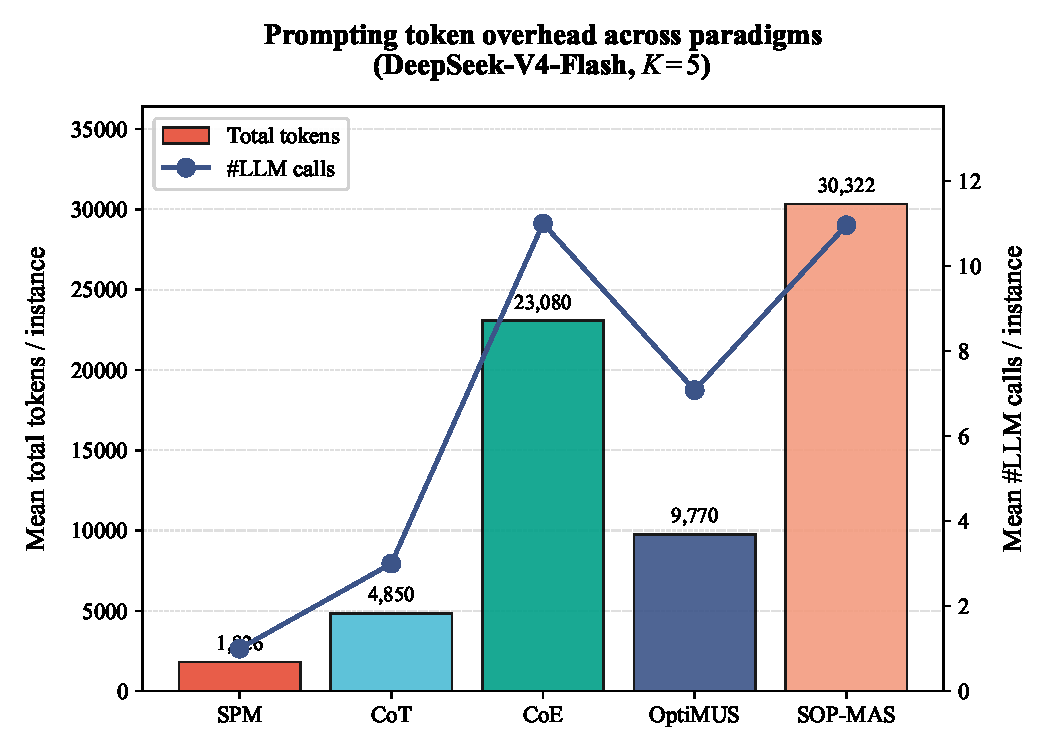
\includegraphics[width=\linewidth]{fig6_token_overhead.pdf}
\subcaption{Token overhead}\label{fig:token_bars}
\end{subfigure}\hfill
\begin{subfigure}[b]{0.49\textwidth}
\centering
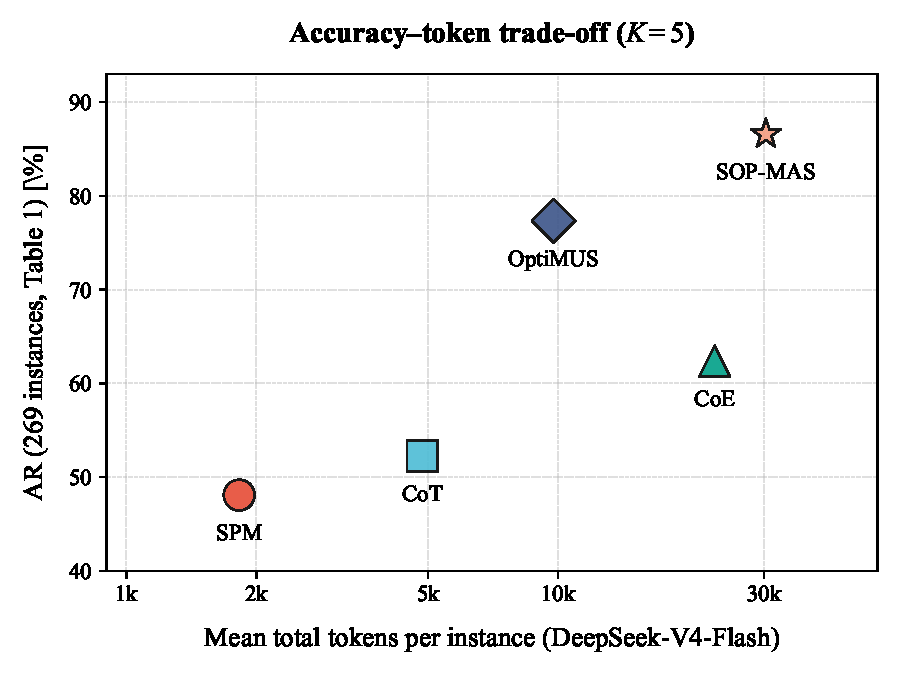
\includegraphics[width=\linewidth]{fig7_token_tradeoff.pdf}
\subcaption{Accuracy--token trade-off}\label{fig:token_tradeoff}
\end{subfigure}
\caption{Prompting token overhead across paradigms (DeepSeek-V4-Flash, $K{=}5$): (a) mean total tokens (bars) and number of LLM calls (line) per instance; (b) AR (cited from Table~\ref{tab:benchmark}) versus mean total tokens, with SOP-MAS at the upper right.}\label{fig:token_overhead}
\end{figure}

\section{Empirical Analysis}

\subsection{Case Setup and Data Sources}\label{sec:case_setup}

This section selects ECR as the empirical testbed because it represents a high-stakes, data-rich problem that demands both mathematical rigor and business interpretability, precisely the dual requirements our SOP-MAS framework is designed to fulfill. Unlike generic optimization benchmarks, real-world ECR involves intricate trade-offs among transportation cost, multimodal transport, and contractual obligations across multiple stakeholders, making it an ideal domain for evaluating whether SOP-MAS-driven modeling can transition from theoretical promise to industrial utility. The empirical analysis examines the Liaoning coastal port cluster in Northeast China, which comprises three seaports with complementary roles: Dalian (international transshipment hub for the northeastern economic region, encompassing Liaoning, Jilin, and Heilongjiang provinces as well as the four eastern leagues of Inner Mongolia), Yingkou (low-cost land transport, forming a dual-core structure with Dalian), and Dandong (logistics gateway for eastern Northeast China). These ports share overlapping hinterlands that form key nodes for sea--rail intermodal transportation (Figure~\ref{fig:port_hinterland_map}).

%% Use figure environment to create figures
%% Refer following link for more details.
%% https://en.wikibooks.org/wiki/LaTeX/Floats,_Figures_and_Captions
\begin{figure}[t]%% placement specifier
%% Use \includegraphics command to insert graphic files. Place graphics files in
%% working directory.
\centering%% For centre alignment of image.
\includegraphics[scale=0.6]{fig5_port_hinterland_map.pdf}
%% Use \caption command for figure caption and label.
\caption{Port hinterland map}\label{fig:port_hinterland_map}
%% https://en.wikibooks.org/wiki/LaTeX/Importing_Graphics#Importing_external_graphics
\end{figure}

A planning horizon of five 7-day periods is adopted. Following \citet{caiJointOptimizationEmpty2024}, the freight rates for empty container transportation by maritime, road, and rail are 0.8, 4.5, and 1.8 CNY/TEU/km, respectively; the leasing cost at seaports is 4,000 CNY/TEU; the holding cost is 10 CNY/TEU/day at seaports and 5 CNY/TEU/day at dry ports; the supply and demand of empty containers at each node per period follow a normal distribution. Inter-node distances and all other parameters are detailed in~\ref{app2}.


\subsection{Problem Description}\label{sec:problem_description}

The ECR network is modeled as a directed graph $G=(\mathcal{N},E)$, where $\mathcal{N}=\mathcal{P}\cup\mathcal{L}$ partitions nodes into the seaport set $\mathcal{P}$ and the dry port set $\mathcal{L}$, and $T=\{1,\ldots,|T|\}$ indexes the planning periods. The edge set $E$ represents repositioning routes among seaports, between seaports and dry ports, and among dry ports. A binary parameter $\lambda_{ij}=1$ indicates that dry port $j$ belongs to the hinterland of seaport $i$; when two dry ports $j_1,j_2\in\mathcal{L}$ share the same affiliated seaport ($\lambda_{ij_1}=\lambda_{ij_2}=1$), direct inter-dry-port repositioning is permitted. The empty container supply $Q_i^t$ at each node derives from inbound laden containers in the preceding period, while outbound laden containers constitute the demand $D_i^t$. Each node has a maximum storage capacity $U_i^{\max}$ and a per-period holding cost $c_i^\text{hold}$. Shortages are met by repositioning from other nodes at unit cost $c_{ijm}^\text{repos}$ via transport mode $m\in\mathcal{M}$ (subject to capacity $F_{ijm}^{\max}$), or by leasing from external providers at cost $c_i^\text{rent}$. The objective is to minimize the aggregate repositioning, storage, and leasing costs over the planning horizon, subject to the following assumptions:

\begin{enumerate}[label=\arabic*)]
 \item Empty containers may be repositioned among seaports, between seaports and dry ports, and among dry ports.
 \item Both seaports and dry ports can store empty containers, subject to maximum capacity.
 \item Container leasing is available in virtually unlimited quantity at each node.
\end{enumerate}

The complete mathematical formulation is provided in~\ref{app3}.

\subsection{Results Analysis}\label{sec:results_analysis}

Based on the ECR problem setting described in Section~\ref{sec:problem_description} and the data presented in Section~\ref{sec:case_setup}, the SOP-MAS framework was employed for end-to-end optimization.

Under the sea–land coordination scenario (Scenario~1), wherein hinterland lateral repositioning is permitted, the optimal total cost over the five-period planning horizon is CNY~1,190,336, comprising repositioning costs of CNY~763,966, holding costs of CNY~30,870, and leasing costs of CNY~395,500, as summarized in Table~\ref{tab:cost_summary}.

To evaluate the benefits of hinterland lateral repositioning, a comparative analysis was conducted under the scenario without inter-dry-port exchange (Scenario~2), as illustrated in Figure~\ref{fig:cost_comparison}. As shown in Table~\ref{tab:cost_summary}, the total cost increases from CNY~1,190,336 to CNY~1,355,388. This increase is primarily driven by the repositioning costs, which rise from CNY~763,966 to CNY~925,238 (a 17.43\% saving under Scenario~1). Within the repositioning category, the sea--land repositioning cost surges from CNY~594,952 to CNY~864,910 (a 31.21\% saving under Scenario~1), as the network must compensate for the loss of hinterland lateral flows (CNY~110,718 reduced to zero) by routing more containers through the sea--dry corridors. Furthermore, the exacerbated difficulty in empty container flows leads to a greater number of containers failing to arrive at shortage seaports in a timely manner, which in turn increases the leasing demand at the affected seaports from CNY~395,500 to CNY~406,000 (a 2.59\% saving under Scenario~1). Overall, enabling hinterland lateral repositioning yields a 12.18\% reduction in total operational costs. \changed{Because the two scenarios differ solely in whether hinterland lateral repositioning is enabled, this entire reduction is the marginal effect attributable to the lateral land route: the CNY~110{,}718 spent on hinterland lateral flows avoids CNY~269{,}958 in sea--land repositioning and CNY~10{,}500 in leasing, yielding a net saving of CNY~165{,}052 after accounting for a CNY~6{,}720 increase in holding cost.}

\begin{table}[htbp]
\centering
\begin{threeparttable}
\caption{Comparison of cost structures under the two scenarios (CNY)}
\label{tab:cost_summary}
\small
\setlength{\tabcolsep}{7pt}
\renewcommand{\arraystretch}{1.20}
\begin{tabular}{@{}l r r r@{}}
\toprule
\textbf{Cost component} & \textbf{Scenario~1} & \textbf{Scenario~2} & \textbf{Change} \\
\midrule
\textbf{Repositioning cost} & \textbf{763,966} & \textbf{925,238} & $-$17.43\% \\
\quad Seaport feeder repositioning & 58,296 & 60,328 & $-$3.37\% \\
\quad Sea--land repositioning & 594,952 & 864,910 & $-$31.21\% \\
\quad Hinterland lateral repositioning & 110,718 & \multicolumn{1}{c}{---} & \multicolumn{1}{c}{---} \\
\addlinespace
Holding cost & 30,870 & 24,150 & +27.83\% \\
\addlinespace
Leasing cost & 395,500 & 406,000 & $-$2.59\% \\
\midrule
\textbf{Total cost} & \textbf{1,190,336} & \textbf{1,355,388} & $-$12.18\% \\
\bottomrule
\end{tabular}
\begin{tablenotes}[flushleft]
 \footnotesize
 \item \textit{Note.} Scenario~1 permits hinterland lateral repositioning; Scenario~2 disables inter-dry-port exchange.
\end{tablenotes}
\end{threeparttable}
\end{table}

Beyond the numerical comparison in Table~\ref{tab:cost_summary}, the \changed{Business Analyst Agent ($a_{\text{BA}}$)} converts the large-scale solver output for Scenario~2 into a structured business report. Specifically, it identifies the total cost as CNY~1,355,388 and attributes 68.26\% to repositioning (CNY~925,238), 29.95\% to leasing (CNY~406,000), and 1.78\% to holding (CNY~24,150). It further highlights the dominant supply and receiving hubs, identifies shortage-prone inland nodes, and recommends prioritizing the Yingkou--Dalian repositioning corridor, securing long-term leasing agreements in inland shortage locations, and clearing stagnant inventories in peripheral nodes. This example illustrates how the \changed{Business Analyst Agent ($a_{\text{BA}}$)} transforms a mathematically optimal solution into an actionable managerial interpretation.

%% Use figure environment to create figures
%% Refer following link for more details.
%% https://en.wikibooks.org/wiki/LaTeX/Floats,_Figures_and_Captions
\begin{figure}[t]%% placement specifier
%% Use \includegraphics command to insert graphic files. Place graphics files in
%% working directory.
\centering%% For centre alignment of image.
\includegraphics[scale=0.5]{fig6_cost_comparison.pdf}
%% Use \caption command for figure caption and label.
\caption{Cost comparison}\label{fig:cost_comparison}
%% https://en.wikibooks.org/wiki/LaTeX/Importing_Graphics#Importing_external_graphics
\end{figure}

\subsection{Formulation Stability Analysis}
This section examines whether the framework produces structurally consistent MIP formulations when applied repeatedly to the same problem instance. The standard benchmark datasets (ComplexOR and NLP4LP) used in Section~4 are designed for correctness evaluation: they involve relatively few variables and constraints, and the resulting formulation space is small. Under such conditions, the Structural-Agreement Rate (SAR)---defined as pairwise agreement of the formulation structure $(n_{\text{vars}}, n_{\text{constrs}}, n_{\text{bin}}, n_{\text{int}}, \text{nnz})$---has limited discriminative power. \changed{Here, $n_{\text{vars}}$ denotes the total number of decision variables, $n_{\text{constrs}}$ the number of constraints, $n_{\text{bin}}$ the number of binary variables, $n_{\text{int}}$ the number of integer variables, and nnz the number of non-zero coefficients in the constraint matrix. Let $F_i=(n_{\text{vars}}^i, n_{\text{constrs}}^i, n_{\text{bin}}^i, n_{\text{int}}^i, \text{nnz}^i)$ denote the formulation structure observed in the $i$-th run that produced a valid formulation. The SAR is then computed as
\begin{equation}
\text{SAR}=\frac{\displaystyle\sum_{1\le i<j\le R'}\mathbf{1}\!\left(F_i=F_j\right)}{\displaystyle\binom{R'}{2}},
\end{equation}
where $R'$ is the number of runs that yielded a formulation structure (excluding only runs that failed before model construction) and $\mathbf{1}(\cdot)$ is the indicator function that equals~1 when the two formulation structures match exactly.} When the formulation space is narrow, most structurally feasible formulations naturally coincide, yielding high SAR values that reflect problem simplicity rather than generation stability. Therefore, the empirical ECR instance used in this section is substantially more complex: 13 nodes (3 seaports and 10 dry ports) over 5 planning periods, yielding a formulation with approximately 975 variables and over 700 constraints in its fully specified form. This instance admits multiple structurally distinct yet feasible representations, where the formulation space is large enough to expose genuine variability in the generation process.

Table~\ref{tab:formulation_stability} summarizes the formulation stability results across two independent trials ($R{=}25$). The ground-truth optimal cost for Scenario~2 is CNY~1,355,388. Three patterns emerge from the results:

\begin{enumerate}
 \item \textbf{Low SAR yet high AR.} The SAR is only 13.7\%, with 8 distinct feasible formulation structures observed across 25 runs. Despite this structural diversity, all feasible runs converge to the same ground-truth optimum. The most frequent structure $(370, 130, 370, 718)$ accounts for 7 of 25 runs, while the remaining runs adopt alternative but mathematically equivalent encodings (e.g., variable upper bounds instead of explicit capacity constraints, or time-window pre-filtering of repositioning arcs). \changed{Here, ``equivalent'' refers to the optimal objective value rather than to solver behavior: the structurally distinct encodings do differ in solve time and simplex iteration count, but these differences are bounded and negligible at this scale, with every feasible variant attaining the optimum within milliseconds.}

 \item \textbf{Compact formulations dominate.} Among the 8 feasible structures, 6 use compact formulations with $n_{\text{vars}} \leq 458$, accounting for 15 of 18 feasible runs. Only 2 structures adopt the expanded formulation ($n_{\text{vars}} = 975$, creating variables for all node pairs), yet both achieve the correct objective by setting non-adjacent arc flows to zero.

 \item \textbf{Error modes are coarse-grained.} In the observed runs, outcomes fall into two broad categories: feasible runs that all achieve the exact optimum, and code-execution failures (e.g., missing Gurobi license, syntax error) that prevent model construction entirely. Across 25 runs, the accuracy rate is 72.0\% (18/25).
\end{enumerate}

\begin{table}[!htbp]
 \centering
 \small
 \renewcommand{\arraystretch}{1.0}
 \caption{Empirical ECR instance formulation stability.}
 \label{tab:formulation_stability}
 \begin{threeparttable}
 \begin{tabular*}{\textwidth}{@{\extracolsep{\fill}}cccccccc@{}}
 \toprule
 ID & $n_{\text{vars}}$ & $n_{\text{constrs}}$ & $n_{\text{int}}$ & nnz & Obj.\ (CNY) & Count & Status \\
 \midrule
 --- & --- & --- & --- & --- & --- & 5 & Error \\
 F1 & 361 & 0 & 361 & 0 & --- & 1 & Error \\
 F2 & 370 & 0 & 370 & 0 & --- & 1 & Error \\
 F3 & 361 & 65 & 361 & 644 & 1,355,388 & 1 & Optimal \\
 F4 & 361 & 130 & 361 & 709 & 1,355,388 & 2 & Optimal \\
 F5 & 370 & 65 & 370 & 653 & 1,355,388 & 3 & Optimal \\
 F6 & 370 & 74 & 370 & 662 & 1,355,388 & 1 & Optimal \\
 F7 & 370 & 130 & 370 & 718 & 1,355,388 & 7 & Optimal \\
 F8 & 458 & 221 & 458 & 884 & 1,355,388 & 1 & Optimal \\
 F9 & 975 & 130 & 975 & 1798 & 1,355,388 & 2 & Optimal \\
 F10 & 975 & 984 & 975 & 2652 & 1,355,388 & 1 & Optimal \\
 \midrule
 \multicolumn{8}{l}{\textbf{AR:} 18/25\,=\,72.0\%; \textbf{SAR:} 26/190\,=\,13.7\%} \\
 \bottomrule
 \end{tabular*}
 \begin{tablenotes}[flushleft]
 \footnotesize
 \item \textit{Note.} \changed{$n_{\text{bin}}=n_{\text{int}}$ for all formulations, as every integer variable in the ECR model is binary; the column is therefore omitted to avoid redundancy.}
 \end{tablenotes}
 \end{threeparttable}
\end{table}

The results reveal that the primary source of instability is \emph{constraint-level encoding variability}: across independent runs, the LLM encodes the same logical constraints in structurally different ways. For example, the storage capacity constraint (``each node has a maximum storage capacity'') is stated explicitly in the problem description. In F7 $(370, 130, 370, 718)$, the most frequent formulation with 7 runs, it appears as a standalone inequality ($I_{i,t} \leq U_i$, where $I_{i,t}$ is the inventory at node $i$ in period $t$ and $U_i$ is the storage capacity); in F5 $(370, 65, 370, 653)$ (3 runs), the same bound is folded into the variable upper bound ($I_{i,t} \in [0, U_i]$) and therefore disappears from the constraint count. Both encodings are mathematically equivalent and yield the same optimum, yet they produce distinct formulation structures. This encoding variability, rather than constraint omission, accounts for most of the observed structural diversity.
\section{Conclusions}

In order to address the limitations associated with MIP, which predominantly relies on domain experts and requires problem-specific customization, this study introduces a decision-support framework titled SOP-MAS. This framework integrates large language models with multi-agent theory. The proposed framework facilitates end-to-end optimization by translating natural language descriptions of business optimization problems into actionable business solutions, thereby substantially reducing the application threshold of MIP. To mitigate hallucination issues and the black-box nature of LLM-based decision-making, this study introduces carefully designed prompts, an orchestrated workflow based on standard operating procedures, and an exception-backtracking mechanism to enhance interpretability.

The effectiveness of the approach was validated through comparisons with multiple baseline methods on the ComplexOR and NLP4LP benchmark datasets, achieving an accuracy of 86.59\%. SOP-MAS was subsequently employed to address the empty container repositioning challenge in the Liaoning coastal port cluster–Northeast hinterland context, leading to a 12.18\% reduction in total operational costs for the shipping company. This application notably curtailed modeling and solution times, expedited prototype development, and furnished scalable decision support amid evolving business rules.

\changed{SOP-MAS is deliberately designed as an expert-in-the-loop decision support system, where human expertise constitutes a core architectural layer. Domain experts provide three essential functions: (i) validation of model assumptions against operational constraints, (ii) business-rule checking for contractual and regulatory compliance, and (iii) strategic acceptance of optimized solutions before deployment.} Several promising directions merit further investigation. First, extending the SOP-MAS framework to more complex optimization paradigms, such as stochastic programming, robust optimization, and multi-objective optimization, would broaden its applicability to real-world ECR scenarios involving demand uncertainty, disruption risks, and conflicting stakeholder objectives. Second, deploying the framework in interactive, human-in-the-loop settings would enable iterative refinement and support a broader set of stakeholders, including seaports, dry ports, shippers, and third-party leasing companies, within the container supply chain. Third, while the evaluation metrics rigorously assess the optimization core of SOP-MAS, the \changed{Business Analyst Agent ($a_{\text{BA}}$)} introduces a qualitatively different output type, namely business interpretation and decision recommendations, that extends beyond solution correctness. Developing dedicated evaluation dimensions for this agent, such as interpretation accuracy, recommendation completeness, and decision actionability, and validating them through structured expert studies with logistics practitioners, would enrich the multi-agent evaluation framework and provide rigorous empirical evidence of the \changed{Business Analyst Agent ($a_{\text{BA}}$)}'s contribution to decision support.

\section*{Data Availability}
The code and data that support the findings of this study are publicly available in the SOP-MAS repository at \url{https://github.com/icsco-mako/sop-mas-ecrp}.



%% The Appendices part is started with the command \appendix;
%% appendix sections are then done as normal sections
\clearpage
\appendix
\section{Agent Prompt Template}\label{app1}
We present the prompt template of the core agent (the \changed{Modeling Expert Agent, $a_{\text{ME}}$}) as a representative example. Complete templates for all agents are available at \url{https://github.com/icsco-mako/sop-mas-ecrp}.

\begin{nolinenumbers}
\begin{promptbox}
\begin{lstlisting}[style=prompttemplate]
# ROLE: Modeling Expert

## INPUT
- Problem description: {problem_description}
- Expert comments: {message_pool}
- Naming convention: {parameter_naming_convention_document}

## TASK
Build a complete mathematical optimization model through:

1. Problem Analysis
 Identify problem type (LP / IP / MIP) from inputs.

2. Model Construction
 (a) Decision Variables
 Define all variables with CamelCase naming.
 Annotate types (Continuous / Integer / Binary).
 (b) Objective Function
 Formulate with explicit unit labels.
 Verify dimensional consistency with constraints.
 (c) Constraints
 Categorize as Resource / Logical / Business.
 List non-negativity constraints separately for
 each variable type; do not combine them.
 Use non-strict inequalities only (<=, >=, =).

3. Validation Rules
 * No new parameters may be introduced.
 * Auxiliary variables are allowed for model clarity.
 * Express all math in LaTeX notation ($x$, $$eq$$).
 * No code generation required.

## OUTPUT FORMAT (Markdown)
# parameters
(list all parameters with symbols and definitions)

# variables
(list all variables with types and dimensions)

# objective
(the objective function in LaTeX)

# constraints
(all constraints in LaTeX, grouped by category)

# ambiguities
(any unclear points from the problem description)
\end{lstlisting}
\end{promptbox}
\captionof{lstlisting}{Representative prompt template for the \changed{Modeling Expert Agent ($a_{\text{ME}}$)}}
\label{lst:me-agent-prompt}
\end{nolinenumbers}
\section{Empirical Case Data}\label{app2}

\begin{table}[htbp]
\centering
\caption{Sea ports repositioning cost and transit time}
\label{tab:seaport_repositioning}
\begin{tabular*}{\textwidth}{@{\extracolsep{\fill}}llllll@{}}
\hline
Seaport & Seaport & Distance & Unit Price & Reposition Cost & Period \\
\hline
Dalian Port & Yingkou Port & 194.1 km & ¥0.8/km & ¥155.28 & 1 \\
Yingkou Port & Dandong Port & 340.4 km & ¥0.8/km & ¥272.32 & 1 \\
Dandong Port & Dalian Port & 315 km & ¥0.8/km & ¥252 & 1 \\
Dalian Port & Dandong Port & 534.5 km & ¥0.8/km & ¥427.6 & 2 \\
Yingkou Port & Dalian Port & 655.4 km & ¥0.8/km & ¥524.32 & 2 \\
Dandong Port & Yingkou Port & 509.1 km & ¥0.8/km & ¥407.28 & 2 \\
\hline
\end{tabular*}
\end{table}

\begin{table}[htbp]
\centering
\caption{Port-hinterland distance matrix (km)}
\label{tab:port_hinterland_distance}
\begin{tabular}{lccc}
\hline
City & {Dalian Port} & {Yingkou Port} & {Dandong Port} \\
\hline
Shenyang & 379.2 & 180.4 & 243.2 \\
Anshan & 298.8 & 102.1 & 236.0 \\
Harbin & 1015.8 & 747.7 & - \\
Changchun & 676.1 & 478.6 & - \\
Tonghua & 623.0 & 439.4 & 275.0 \\
Jilin & 520.0 & 540.0 & - \\
Tongliao & 460.0 & 380.0 & - \\
Chifeng & 580.0 & 620.0 & - \\
Daqing & 870.0 & - & - \\
Qiqihar & 930.0 & - & - \\
\hline
\end{tabular}
\end{table}


\begin{table}[htbp]
\centering
\caption{Inter-dry port distances (km)}
\label{tab:inter_dryport_distance}
\begin{tabular*}{0.65\textwidth}{@{\extracolsep{\fill}}llc@{}}
\hline
Dry port & Dry port & Distance \\
\hline
Shenyang & Anshan & 85 \\
Shenyang & Changchun & 278 \\
Shenyang & Tonghua & 208 \\
Shenyang & Jilin & 343 \\
Shenyang & Tongliao & 224 \\
Shenyang & Chifeng & 376 \\
Anshan & Tonghua & 256 \\
Anshan & Tongliao & 285 \\
Anshan & Chifeng & 361 \\
Harbin & Changchun & 232 \\
Harbin & Jilin & 211 \\
Harbin & Daqing & 154 \\
Changchun & Jilin & 100 \\
Changchun & Tongliao & 247 \\
Changchun & Daqing & 301 \\
Changchun & Qiqihar & 400 \\
Jilin & Daqing & 327 \\
Jilin & Qiqihar & 440 \\
Tongliao & Chifeng & 311 \\
Daqing & Qiqihar & 119 \\
\hline
\end{tabular*}
\end{table}

\begin{table}[htbp]
\centering
\caption{Empty container demand and supply at each node (TEU)}
\label{tab:ec_demand_supply}
\begin{tabular*}{0.65\textwidth}{@{\extracolsep{\fill}}llc@{}}
\hline
Port/EC volume (TEU) & EC demand & EC supply \\
\hline
Shenyang & $(5000, 100^2)$ & $(4150, 100^2)$ \\
Anshan & $(1250, 50^2)$ & $(1350, 50^2)$ \\
Harbin & $(800, 40^2)$ & $(800, 40^2)$ \\
Changchun & $(500, 20^2)$ & $(500, 20^2)$ \\
Tonghua & $(500, 20^2)$ & $(500, 20^2)$ \\
Jilin & $(500, 20^2)$ & $(500, 20^2)$ \\
Tongliao & $(500, 20^2)$ & $(500, 20^2)$ \\
Chifeng & $(100, 20^2)$ & $(100, 20^2)$ \\
Daqing & $(300, 20^2)$ & $(300, 20^2)$ \\
Qiqihar & $(100, 20^2)$ & $(100, 20^2)$ \\
\hline
\end{tabular*}
\end{table}
\clearpage

\section{ECR Mathematical Model}\label{app3}
As one of our core contributions is the automatic synthesis of publication-ready mathematical formulations, we present the complete ECR model generated by the SOP-MAC framework below. The main text summarizes the problem setting, key decision logic, and operational assumptions in Section~\ref{sec:problem_description}, while this appendix provides the full formulation for readers seeking model-level detail.
\begin{nolinenumbers}
\begin{promptbox}
\begin{lstlisting}[style=prompttemplate]
### **Parameters**

- $ \mathcal{P} $: Set of seaports
- $ \mathcal{L} $: Set of inland ports
- $ \mathcal{N} = \mathcal{P} \cup \mathcal{L} $: Set of nodes
- $ \mathcal{M} $: Set of transportation modes (e.g., ship, truck, train)
- $ T $: Set of time periods ($ T = \{1, 2, \ldots, |T|\} $)
- $ \lambda_{ij} \in \{0,1\} $: $ = 1 $ if inland port $ j $ belongs to hinterland of seaport $ i $
- $ \alpha_{j_1 j_2} \in \{0,1\} $: $ = \max_{h \in \mathcal{P}} (\lambda_{h j_1} \lambda_{h j_2}) $, inland port collaboration indicator
- $ Q_i^t \geq 0 $: Empty container supply at node $ i \in \mathcal{N} $ in period $ t $
- $ D_i^t \geq 0 $: Empty container demand at node $ i \in \mathcal{N} $ in period $ t $
- $ U_i^{\max} > 0 $: Maximum storage capacity at node $ i \in \mathcal{N} $
- $ c_i^{\text{hold}} > 0 $: Unit inventory holding cost at node $ i \in \mathcal{N} $
- $ c_{ijm}^{\text{repos}} > 0 $: Unit repositioning cost for moving an empty container from $ i $ to $ j $ via mode $ m $
- $ F_{ijm}^{\max} \geq 0 $: Maximum transportation capacity on arc $ (i,j) $ using mode $ m $
- $ c_i^{\text{rent}} > 0 $: Unit container rental cost at node $ i \in \mathcal{N} $
- $ \tau_{ij} \geq 1 $: Repositioning lead time (in periods) for shipments from seaport $ i $ to seaport $ j $ (defined only for $ i,j \in \mathcal{P} $)
- $ w_i^0 \geq 0 $: Initial inventory at node $ i $ at the beginning of period 1
- $ M = \sum_{t \in T} \sum_{i \in \mathcal{N}} D_i^t $: A sufficiently large constant

### **Decision Variables**

- $ w_i^t \geq 0 $: Inventory of empty containers at node $ i \in \mathcal{N} $ at the end of period $ t $ (continuous)
- $ x_{ijm}^t \geq 0 $: Quantity of empty containers repositioned from node $ i $ to node $ j $ via mode $ m $ in period $ t $ (continuous)
- $ r_i^t \geq 0 $: Quantity of containers rented at node $ i \in \mathcal{N} $ in period $ t $ (continuous)

### **Objective Function**
Minimize total operational cost (repositioning + holding + rental):
$$
\min \sum_{t \in T} \left(
\sum_{i \in \mathcal{N}} \sum_{j \in \mathcal{N}} \sum_{m \in \mathcal{M}} c_{ijm}^{\text{repos}} x_{ijm}^t
+ \sum_{i \in \mathcal{N}} c_i^{\text{hold}} w_i^t
+ \sum_{i \in \mathcal{N}} c_i^{\text{rent}} r_i^t
\right)
$$

### **Constraints**

#### **1. Flow Balance Constraints**
**For seaport nodes $ i \in \mathcal{P} $** (incorporating hinterland affiliation and lead time):
$$
w_i^{t-1} + Q_i^t + r_i^t + \sum_{\substack{j \in \mathcal{P} \\ m \in \mathcal{M} \\ t > \tau_{ji}}} x_{jim}^{t - \tau_{ji}} + \sum_{\substack{j \in \mathcal{L} \\ m \in \mathcal{M} \\ \lambda_{ij} = 1}} x_{jim}^{t} = D_i^t + \sum_{\substack{j \in \mathcal{P} \\ m \in \mathcal{M}}} x_{ijm}^{t} + \sum_{\substack{j \in \mathcal{L} \\ m \in \mathcal{M} \\ \lambda_{ij} = 1}} x_{ijm}^{t} + w_i^{t} \quad \forall t \in T
$$

**For inland port nodes $ j \in \mathcal{L} $** (strict hinterland restriction; all repositioning is instantaneous):
$$
w_j^{t-1} + Q_j^t + r_j^t + \sum_{\substack{i \in \mathcal{P} \\ m \in \mathcal{M} \\ \lambda_{ij} = 1}} x_{ijm}^{t} + \sum_{\substack{i \in \mathcal{L} \\ m \in \mathcal{M} \\ \alpha_{ij} = 1}} x_{ijm}^{t} = D_j^t + \sum_{\substack{i \in \mathcal{P} \\ m \in \mathcal{M} \\ \lambda_{ij} = 1}} x_{jim}^{t} + \sum_{\substack{i \in \mathcal{L} \\ m \in \mathcal{M} \\ \alpha_{ij} = 1}} x_{jim}^{t} + w_j^{t} \quad \forall t \in T
$$

#### **2. Hinterland Logic Constraints**
**Seaport and inland port repositioning** (forbidden outside designated hinterlands):
$$
x_{ijm}^t = 0 \quad \forall i \in \mathcal{P}, j \in \mathcal{L}, m \in \mathcal{M}, t \in T, \text{ if } \lambda_{ij} = 0
$$

$$
x_{jim}^t = 0 \quad \forall i \in \mathcal{P}, j \in \mathcal{L}, m \in \mathcal{M}, t \in T, \text{ if } \lambda_{ij} = 0
$$

**Inland port and inland port repositioning** (permitted only if ports share a common seaport hinterland):
$$
x_{j_1 j_2 m}^t \leq M \cdot \alpha_{j_1 j_2} \quad \forall j_1, j_2 \in \mathcal{L}, m \in \mathcal{M}, t \in T
$$

#### **3. Physical Limit Constraints**
**Transportation capacity constraints** (for all arcs):
$$
x_{ijm}^t \leq F_{ijm}^{\max} \quad \forall i,j \in \mathcal{N}, m \in \mathcal{M}, t \in T
$$

**Storage capacity constraints** (for all nodes):
$$
w_i^t \leq U_i^{\max} \quad \forall i \in \mathcal{N}, t \in T
$$

**Non-negativity constraints** (for all variables):
$$
w_i^t \geq 0, \quad x_{ijm}^t \geq 0, \quad r_i^t \geq 0 \quad \forall i,j \in \mathcal{N}, m \in \mathcal{M}, t \in T
$$

\end{lstlisting}
\end{promptbox}
% \captionof{lstlisting}{Complete ECR mathematical formulation generated by SOP-MAS}
\label{lst:ecr-mathematical-model}
\end{nolinenumbers}

\section{Case Analysis of Formulation Variability}\label{app4}

To ground the aggregate findings of the formulation stability experiment (Section~6.3), we analyze a representative run (F10) from the 25 independent trials, which is correct despite a structurally unusual formulation.

F10 yields the structure $(975,\;984,\;975,\;2652)$, the largest among all 25 runs, yet achieves the ground-truth optimum of CNY~1,355,388. The key difference is in how repositioning variables are defined. Instead of creating variables only for adjacent arcs (the approach taken by F7, the most common formulation with 7 runs), the generated code enumerates \emph{all} node pairs and enforces zero flow on non-adjacent arcs through big-$M$ constraints:

\begin{nolinenumbers}
\begin{promptbox}
\begin{lstlisting}[style=prompttemplate]
# Variables: reposition for ALL node pairs (13x13x5 = 845)
reposition = m.addVars(N, N, T, vtype=GRB.INTEGER, lb=0)
inventory = m.addVars(N, T, vtype=GRB.INTEGER, lb=0) # 65
leasing = m.addVars(N, T, vtype=GRB.INTEGER, lb=0) # 65

# Big-M: force zero on non-adjacent arcs
bigM = max(sum(supply[i]) + sum(demand[i]) for i in range(N)) * 10
for i in range(N):
 for j in range(N):
 for t in range(T):
 m.addConstr(reposition[i,j,t] <= adj_matrix[i][j] * bigM)
 if t + tau_matrix[i][j] >= T: # arrival beyond horizon
 m.addConstr(reposition[i,j,t] == 0)
\end{lstlisting}
\end{promptbox}
\label{lst:case-a-expanded}
\end{nolinenumbers}

This encoding produces $845 + 65 + 65 = 975$ variables and $65 + 65 + 845 + 9 = 984$ constraints (balance, capacity, adjacency, and time-window), with 2,652 non-zero coefficients. Despite the structural inflation, the solver correctly identifies that all non-adjacent arc flows must be zero and converges to the same optimum as compact formulations. This case illustrates that LLM-generated formulations can be \emph{structurally different yet mathematically equivalent}: the choice of encoding strategy (full enumeration with big-$M$ vs.\ sparse variable filtering) does not affect solution correctness.

\newpage
%% For citations use:
%% \cite{<label>} ==> [1]

%%
%% If you have bib database file and want bibtex to generate the
%% bibitems, please use
%%
\bibliographystyle{elsarticle-num-names}
\bibliography{ref_sop_mac}

%% else use the following coding to input the bibitems directly in the
%% TeX file.

%% Refer following link for more details about bibliography and citations.
%% https://en.wikibooks.org/wiki/LaTeX/Bibliography_Management



%% \begin{thebibliography}{00}

%% For numbered reference style
%% \bibitem{label}
%% Text of bibliographic item

%% \bibitem{lamport94}
%% Leslie Lamport,
%% \textit{\LaTeX: a document preparation system},
%% Addison Wesley, Massachusetts,
%% 2nd edition,
%% 1994.

%% \end{thebibliography}
\end{document}

\endinput
%%
%% End of file `elsarticle-template-num-names.tex'.
